% -*- TeX:UTF-8 -*-
%%
%% KAIST 학위논문양식 LaTeX용 (ver 0.4) 예시
%%
%% @version 0.4
%% @author  채승병 Chae,Seungbyung (mailto:chess@kaist.ac.kr)
%% @date    2004. 11. 12.
%%
%% @requirement
%% teTeX, fpTeX, teTeX 등의 LaTeX2e 배포판
%% + 은광희 님의 HLaTeX 0.991 이상 버젼 또는 홍석호 님의 HPACK 1.0
%% : 설치에 대한 자세한 정보는 http://www.ktug.or.kr을 참조바랍니다.
%%
%% @note
%% 기존에 널리 쓰여오던 차재춘 님의 학위논문양식 클래스 파일의 형식을
%% 따르지 않고 전면적으로 다시 작성하였습니다. 논문 정보 입력부분에서
%% 과거 양식과 다른 부분이 많으니 아래 예시에 맞춰 바꿔주십시오.
%% 버그 리포트는 http://gsa.kaist.ac.kr/thesis-form으로 보내주십시오.
%%
%% @acknowledgement
%% 본 예시 논문은 물리학과 박사과정 김용현 님의 호의로 제공되었습니다.
%%
%% -------------------------------------------------------------------
%% @information
%% 이 예제 파일은 hangul-ucs를 사용합니다. UTF-8 입력 인코딩으로
%% 작성되었습니다. hlatex의 hfont는 이용하지 않습니다. --2006/02/11

% @class kaist.cls
% @options [default: doctor, korean, final]
% - doctor: 박사과정 | master : 석사과정
% - korean: 한글논문 | english: 영문논문
% - final : 최종판   | draft  : 시험판
% - pdfdoc : 선택하지 않으면 북마크와 colorlink를 만들지 않습니다.
\documentclass[master,english,final]{kaist-ucs}

% kaist.cls 에서는 기본으로 dhucs, ifpdf, graphicx 패키지가 로드됩니다.
% 추가로 필요한 패키지가 있다면 주석을 풀고 적어넣으십시오,
%\usepackage{...}
\usepackage{color}
\usepackage{amsmath}
\usepackage{graphicx}
\usepackage{pdflscape}
\usepackage{hyperref}
\usepackage{multirow}
\usepackage{subfig}

% @command title 논문 제목
% @options [default: (none)]
% - korean: 한글제목 | english: 영문제목
\title[korean] {이족 보행 동역학의\linebreak 생체 역학적인 접근방법}
%\title[english]{Spectral-based Shape Correspondence \linebreak with Diffusion Geometry}
\title[english]{A Biomechanical Approach to Biped Dynamics}

% @note 표지에 출력되는 제목을 강제로 줄바꿈하려면 \linebreak 을 삽입.
%       \\ 나 \newline 등을 사용하면 안됩니다. (아래는 예시)
%\title[korean]{탄소 나노튜브의 물리적 특성에 대한\linebreak 이론 연구}
%\title[english]{Theoretical study on physical properties of\linebreak
%                carbon nanotubes}

% @command author 저자 이름
% @param   family_name, given_name 성, 이름을 구분해서 입력
% @options [default: (none)]
% - korean: 한글이름 | chinese: 한문이름 | english: 영문이름
\author[korean] {김}{거 엽}
\author[chinese]{金}{거 엽}
\author[english]{Kim}{Geo Yeob}

% @command advisor 지도교수 이름 (복수가능)
% @usage   \advisor[options]{...한글이름...}{...영문이름...}{signed|nosign}
% @options [default: major]
% - major: 주 지도교수  | coopr: 공동 지도교수
\advisor[major]{신 성 용}{Shin, Sung Yong}{signed}
%\advisor[coopr]{홍 길 동}{Gil-Dong Hong}{nosign}

% @command department 학과이름 - 아래 표에 따라 코드를 입력
%
% 물리 PH
% 수리과학 MAS
% 화학 CH
% 생명과학 BS
% 바이오및뇌공학 BiS
% 의과학대학원 MSE
% 의과학학제 BM
% 기계공학 ME
% 항공우주공학 AE
% 건설 및 환경공학 CE
% 산업디자인 ID
% 생명화학공학 CBE
% 신소재공학 MS
% 원자력 및 양자 NQE
% 자동차기술대학원 AT
% 전기및전자공학 EE
% 전산학 CS
% 산업 및 시스템공학 IE
% 반도체학제 STE
% 소프트웨어 프로그램 SEP
% 정보통신학제 TE
% 고분자학학제 PSE
% 과학기술학학제 STS
% 나노과학기술학제 NT
% 로봇공학학제 RE
% 문화기술학제 CT
% 환경·에너지공학학제 ENV
% e-매뉴팩쳐링리더십학제 EML
% 문화기술대학원 GCT
% 경영공학 MT
% 테크노경영 TM
% 금융 FIN

\department{CS}

% @command studentid 학번
\studentid{20084004}

% @command referee 심사위원 (석사과정 3인, 박사과정 5인)
\referee[1]{신 성 용}
\referee[2]{조 성 호}
\referee[3]{최 성 희}

% @command approvaldate 지도교수논문승인일
% @param   year,month,day 연,월,일 순으로 입력
\approvaldate{2010}{12}{23}

% @command refereedate 심사위원논문심사일
% @param   year,month,day 연,월,일 순으로 입력
\refereedate{2010}{12}{23}

% @command gradyear 졸업년도
\gradyear{2011}

%\addtolength{\textwidth}{0.6in}
%\addtolength{\hoffset}{-0.4in}
%\addtolength{\textheight}{1.9in}
%\addtolength{\voffset}{-0.8in}

% 본문 시작
\begin{document}
%\begin{CJK*}[HL]{KS}{}

\begin{abstract}
Physically-based models have been adopted widely for character animtion.
Originated from robotics, biped models for character animation
also took a form of robots. The robot-like biped models have joint motors,
so that the motors are controlled to rotate bodies to make desired poses.

In this thesis, we present a biped model based on the biomechanical information that
human movement is controlled with tensions of muscle fibers attached
to skeletal structures instead of actuated motors on joints which do not even exist in
a human body.
With the proposed biped model, we designed a locomotion tracker
that follows given motion trajectories by optimizing the muscle fiber tensions.


\noindent
\\Keywords: character animation, dynamics, biped model, biomechanics

%Relative joint angles between two bodies can be controlled using its motor attached to them,
%however, the global orientation and position of the biped cannot be controlled since
%they have no controllable elements exist.
\end{abstract}


% 목차 (Table of Contents) 생성
\tableofcontents

% 표목차 (List of Tables) 생성
\listoftables

% 그림목차 (List of Figures) 생성
\listoffigures

% 위의 세 종류의 목차는 한꺼번에 다음 명령으로 생성할 수도 있습니다.
%\makecontents

\chapter{Introduction}
\section{Research motivation}
As an integral part of creating animations and video games,
bipedal character animation techniques have drawn much attention from
both academia and industry. Physically-simulated approaches have been
adopted to synthesize realistic and physically correct motions
automatically instead of relying on labor-intensive key-frame animation
techniques. In these approaches, a character is designed and controlled
as a consistent dynamic model, by representing it as an articulated
figure. This model consists of a set of body segments each being
considered as a rigid body and joints connecting these segments.
This kind of models is used widely due to their adequacy to formulating
equations of motion.
The joints used in the model are considered as rigid joints,
that is, each of them connects the two rigid bodies with certain DOFs.
Typically, translational DOFs are not used for joints to disallow dislocation.
For example, hinge joints with one DOF are used at knees or elbows and
ball joints with three DOFs are used at hips. Actuation on joints may change
the angle between bodies. Thus it is natural to call this kind of joints
\emph{actuated motor joints}. Motions can be created by
controlling these motor joints properly. This approach is
commonly used in robotics~\cite{sardain, goswami}.

The concept of actuated motor joints is unrealistic in the perspective of
biomechanics. No human being has such motors in their joints.
Humans control their legs or arms by pulling bones using attached
muscles. Although the whole mechanism is quite complicated,
the structure of human muscle fibers is well-known, and biomechanical
experimental results are available concerning the most basic human actions
such as walking and jumping \cite{citeulike:2547705, citeulike:7093575}.

This thesis presents a biomechanical approach to biped dynamics. We
introduce muscle fibers as the only actuating elements
of a bipedal character and get rid of all rigid motor joints in previous biped
models. Consequently, joints are not rigid anymore in our approach.
We use ligaments in the place of joints
to hold the bodies firmly but not rigidly. This substitution
simulates human cartilages, which provide a shock absorption
system to sustain stability when external or internal disturbances are applied~\cite{shock}.
We control the rigid bodies with a set of muscle fibers each of which are modeled as
a spring-damper system. Every muscle fiber has a linear actuator and
motions are created by controlling the actuator.

\section{Outline}

We model a character which consists of rigid bodies and muscle fibers.
With this biomechanical model we design a reference trajectory tracker
following given trajectories.

More specifically, a biomechanical biped model is defined as $B = (\mathcal{B}, \mathcal{M}, \mathcal {J})$ where
$\mathcal{B}$ is a set of rigid bodies representing human body parts,
$\mathcal{M}$ is a set of muscle fibers and $\mathcal{J}$ is a set of
soft joints. For a given sequence of biped poses $\bar{\chi}$,
that is a reference motion, muscle actuation forces on
each muscle fiber are calculated to make a simulated biped pose
$\chi^{(l+1)}$ as close as possible to
$\bar{\chi}^{(l+1)}$ where $l$ is an index of current simulation time step.
This process is depicted in \ref{overview2}.
Note that the simulated biped pose $\chi^{(l+1)}$ cannot be chosen arbitrarily,
but should strictly obey the equations of motion. Also, there will be intermittent contacts
between feet and the ground floor during locomotion, which will cause normal forces and frictional forces on
the biped. Therefore, it is important to take account of these dynamics constraints to get physically-valid
motions.


\begin{figure}[h!]
\label{probdef}
  \centering
  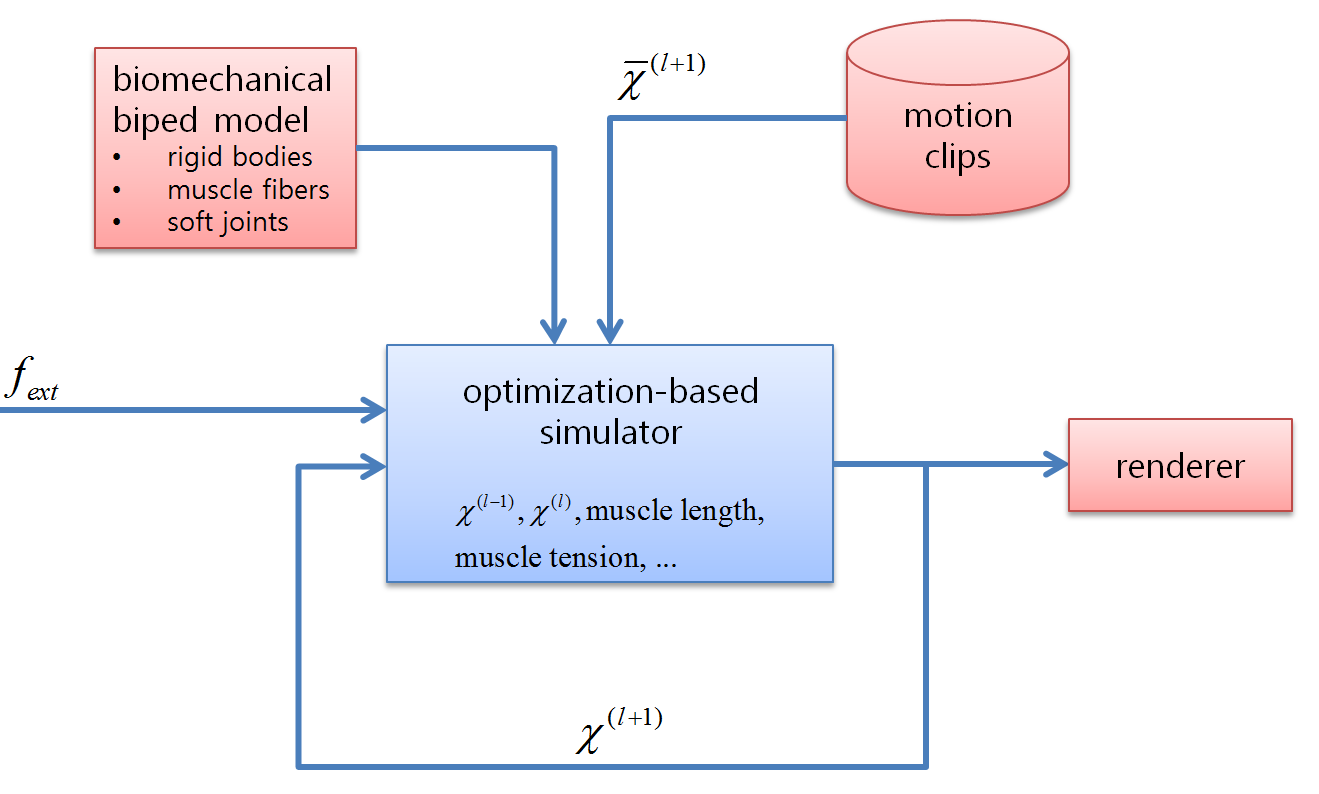
\includegraphics[width=0.75\textwidth]{overview2}
  \caption{Simulation outline}
  \label{overview2}
\end{figure}

This thesis is organized as follows. Chapter 2 describes related work,
focused on physically-based character animation and biomechanics modeling.
In Chapter 3 we describe more details on our biomechanical biped simulation system
including a muscle fiber model and a soft joint model.
An optimization-based reference tracking controller for the biped model
is presented in Chapter 4. We present results of tracking simulation in Chapter 5,
and conclude the paper in Chapter 6.

\chapter{Related work}

\section{Physically-based character animation}
Designing and controlling a physically simulated character is a long-standing
challenge in robotics and computer graphics. A physically
synthesized motion that actively responds to the environment is quite
promising because it is time-consuming to create a natural animation by handcraft keyframing.
Although the combination of motion capture data and manual keyframing
shows a quality of motion, it is not straightforward to make a character
interacts with its environment if a pre-recorded motion clip is used.
This issue could be addressed by combining  a character animation system with physical simulation.
However, there has not yet been an ultimate solution for controlling
a simulated character motion.

Motion controllers were proposed based on the fact
that the ground reaction forces or contact forces affect the global
DOFs of the character significantly \cite{SCA07:249-258:2007, journals/tog/MuicoLPP09}.
Muico and his colleagues
presented a contact-aware controller \cite{journals/tog/MuicoLPP09}.
This approach is
heavily based on the theory of optimal control \cite{lewis}.
The linear quadratic regulator (LQR) was modified to consider the ground reaction forces.
We also take the contact forces into account but in a different way.
We estimate the contact forces using a penalty-based method and adopt an optimization
framework to take account these for calculating the actuation forces of muscle fibers.

Yin and her colleagues
presented a proportional-derivative (PD) control framework \cite{journals/tog/YinLP07}.
They used a finite state machine (FSM) in which target poses are defined
for each state. Considering the complexity of a biped dynamics model,
the structure of controller is simple and robust to external disturbances.
Since they do not consider energy efficiency or passive forces during
control, the animation shows some stiff behavior.
More elaborate animation would be achieved by increasing
the number of states in the FSM. However, this is not a practical alternative
since the number of parameters is proportional to the number of states.

Optimization-based approaches have been employed to address many challenges
in biped control such as high dimensionality, under-actuated joint control and
nonlinearity~\cite{journals/tog/MacchiettoZS09, journals/tog/MuicoLPP09, park}.
Most of these approaches determined joint torques to make a desired pose or
a sequence of desired poses.
Instead of finding the joint torques, Jain and his colleagues formulated
an optimization problem which finds joint angles directly \cite{Jain:09:OIM}.
The joint torques
are implicitly calculated during optimization. The advantage of
this approach is to easily design various types of objectives such as
moving a hand to nearby wall or placing a swing foot to a certain place.
However, it is not intuitive to use a torque-based optimization formulation
for biped control.
We take a similar formulation to find rigid body positions
and orientations rather than joint angles based on optimization.

%------%
\section{Biomechanical model}

We model a biped figure by abstracting the biomechanical configuration
of human bodies.
Researchers in biomechanical engineering dealt with the movement
disorder and biomedical applications such as artificial joints~\cite{svsjan}.
There was rich work which use a model similar to
a real human body since it is important to study the mechanism of underlying
structure of human body in such field \cite{vr-305, neptune}.

Thelen and his colleagues presented
an algorithm to compute muscle excitation patterns that produce
coordinated movements of muscle-actuated dynamic models \cite{Thelen2003321}.
They simulated
the pedaling motion of a person on a bicycle while fixing the upper body to investigate the excitation
pattern of 30 muscle fibers on both legs which significantly affecting leg movements.

An anatomy-based approach to muscle simulation was presented by Dong and his colleagues~\cite{10.1109/2945.998668}.
They dealt with the problem of muscle modeling in order to provide models for human musculature based
on real morphological structures. Their main focus was placed on visualizing muscle forms and actions in
great details.

Liu and her colleagues tried to exploit the passive characteristics of
real muscle fibers by employing torsion springs in joints \cite{Liu:2005:LPB}.
However, the muscle actuation was still done by joint motors, and a musculoskeletal
structure was not discussed at all.

On the other hand, Lee and his colleagues accurately modeled human muscles on the upper body
to simulate the physics-based deformations of the soft tissues \cite{Lee:2009:CBM:1559755.1559756}.
They also designed an animation controller that computes the muscle activation signals to follow target poses
specified by an animator. Their model was heavily focused on a realistic musculoskeletal
model and skin deformations for the upper body.
We present a simplified biomechanical biped model for synthesizing character animation,
but not for visualizing or rendering skin deformations.

For human musculoskeletal structures, we mainly referred to an article on Wikipedia \cite{Wikipedia},
Google Body Browser~\cite{bodybrowser} and a textbook written by Martini~\cite{martini}.
We also adopt a well-known mathematical model of muscle fibers
called a Hill-type model~\cite{hill, Lee:2006:HUB:1141911.1142013}.


%The action for each muscle groups can be anticipated by adopting the
%fact regarding to gait phases \cite{perry}. The gait phases are the essential component
%when analyzing a person's walking pattern. It directly identifies the
%functional significance of the different motions occurring at the
%individual joints. While controlling the character we
%can determine the current gait phase. For each gait phase,
%a subset of the entire muscle fibers is selected to be actuated
%and the others will be unactuated.

%The muscle fiber model we use is composed of two springs and a damper.
%This simple muscle model is explained in detail in the supplementary
%documents [SHADMEHR]. In the document they assume that spring stiffness constants
%and viscosity of the damper are constants. Some studies suggest that animals
%vary stiffness according to the specific locomotion task.[FARLEY]
%Since the model consists of springs we definitely need rest lengths for that
%springs. However rest lengths are not simply defined on real muscles.
%[...]


\chapter{Biomechanical biped system model}

\section{Overview}

Modeling a precise and realistic human musculoskeletal structure for physics simulation
is a challenging problem because there is a large number of muscles and bones in a human body.
Besides, their features, shapes and structures vary widely and are hard to be modeled
accurately.
Our main interest lies on how to design a biped figure actuated by skeletal muscles with reasonable
simplification, which is suitable for character animation.
Skeletal muscles on a human body are depicted in Figures \ref{skelmus1} and \ref{skelmus2}.

\begin{figure}[h!]
  \centering
  \includegraphics[width=3.5in]{muscles_anterior_labeled}
  \caption{Human skeletal muscles (anterior)}
  \label{skelmus1}
\end{figure}

\begin{figure}[h!]
  \centering
  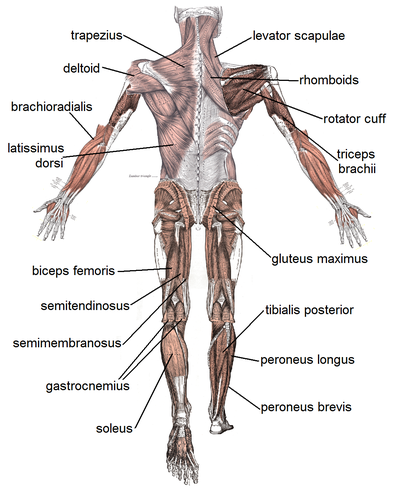
\includegraphics[width=3.5in]{Muscle_posterior_labeled}
  \caption{Human skeletal muscles (posterior)}
  \label{skelmus2}
\end{figure}
\noindent

We introduce anatomical terminologies about muscles to clarify our abstraction of modeling.
Each labeled muscle indicates a \textit{muscle body} or just \textit{muscle}. Also a muscle body
is a bundle of \textit{fascicles}. A fascicle is a bundle of skeletal muscle fibers
surrounded by a connective tissue. We simplify these hierarchical structures of muscles and
assume that each muscle body can be modeled as a certain number of muscle fibers.

In this work, we concentrate on modeling muscles related to legs which mainly contribute to locomotion
such as sartorius, gluteus maximus, quadriceps and so on.
Muscles used in our biped model are listed in Table \ref{musclelist}.

\begin{table}[h!]
\centering
  \begin{tabular}{lccl}
  name                            &  origin       &insertion& action \\
  \hline
  gluteus maximus                 &  15b          & 16b     & extend thigh\\
  gluteus medius                  &  1b           & 2b      & abduct thigh\\
  semimembranosus                 &  13a          & 8b      & flex knee \\
  semitendinosus                  &  11b          & 7b      & flex knee \\
  biceps femoris (long head)      &  14b          & 3b      & flex knee \\
  biceps femoris (short head)     &  14b          & 5b      & flex knee \\
  sartorius                       &  1a           & 10a     & flex thigh \\
  adductor longus                 &  3a           & 5a      & adduct thigh \\
  adductor magnus                 &  12b          & 10b,15b & adduct thigh \\
  gracilis                        &  3a           & 9a      & adduct thigh, flex knee \\
  rectus femoris                  &  2a           & 7a      & extend knee, flex thigh \\
  vastus medialis                 &  5a           & 8a      & extend knee \\
  vastus lateralis                &  4a           & 6a      & extend knee\\
  gastrocnemius                   &  4b, 9b       & 6b      & plantar flex foot, flex knee\\
  \hline
\end{tabular}
\caption[Muscles on a leg used in our model]
{Muscles on a leg used in our model: The location of origin and insertion
is described in Figure~\ref{fig:musclepoints} (a) and (b). For instance, the origin of
sartorius is located at mark 1 on Figure~\ref{fig:musclepoints} (a).}
\label{musclelist}
\end{table}

\begin{figure}[h!]
  \centering
  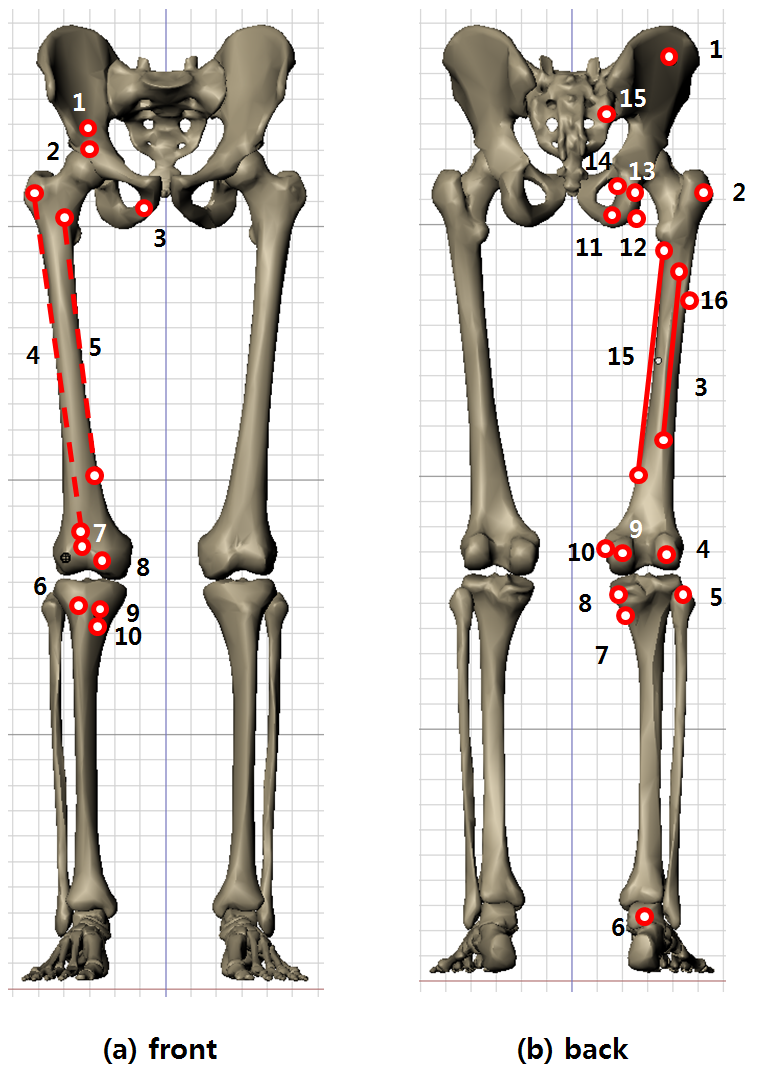
\includegraphics[width=3in]{musclepoints}
  \caption[Muscle origin and insertion points]
  {Muscle origin and insertion points: The dashed lines in (a) denote lines at the back of the femur.}
   \label{fig:musclepoints}
\end{figure}

We greatly simplify the real human musculoskeletal structure to make biomechanical biped modeling tractable.

First, we assume that each muscle body is composed of a small number of muscle fibers.
For example, one end of the biceps femoris is connected to the upper part of
the femur and the tuberosity of ischium (heap).
The other end is connected to the upper part of the fibula. Thus, we model
the muscle using two muscle fibers, which connect the femur and fibula and the heap and fibula,
respectively (Figure \ref{muscleabs} (a)).
When a muscle is attached to a large area on bones, we can use multiple muscle fibers
in the certain area to model it. For example, the quadriceps femoris connects
the tibial tuberosity (knee side of tibia)
and femur. This muscle is attached to the femur in a wide area. In this case,
we use multiple muscle fibers to model the muscle (Figure \ref{muscleabs} (b)).

Second, a muscle is in fact a soft deformable body so as to be deformed freely
with respect to configurations of attached bones or exerted forces. Unlike in applications
such as skin deformations or accurate surgery simulations,
a muscle fiber is treated as a piston in our model, both ends of which are rigidly connected to bones
(modeled as rigid bodies) with ball joints as depicted in Figure \ref{muscleabs} (c) and (d).
Therefore, muscle deformation is not considered in our model.

Third, a detailed bone geometry is not considered on joints.
For example, a hip joint is formed by the articulation of the rounded head of the femur and
the cup-like acetabulum of the pelvis. Instead of modeling each skeleton's exact shape,
we use a box-shaped rigid bodies for representing body segments and assume bones lies
in the rigid bodies.

Fourth, certain bones are removed or merged into other bones for simplicity.
For example, we do not model every fingers or toes with individual bones.
There are two bones called the tibia and the fibula on each calf.
However, we removed the fibula because its feature is lost in humans~\cite{nofibula}.
Patella bones are omitted and fixed on the knee side of the femur.

We model a body segment as a rigid body. One or more bones in human skeleton are
wrapped with a rigid body. Since we model the lower extremity of the biped,
we use a head-arm-trunk (HAT) model.


\begin{figure}[h!]
  \centering
  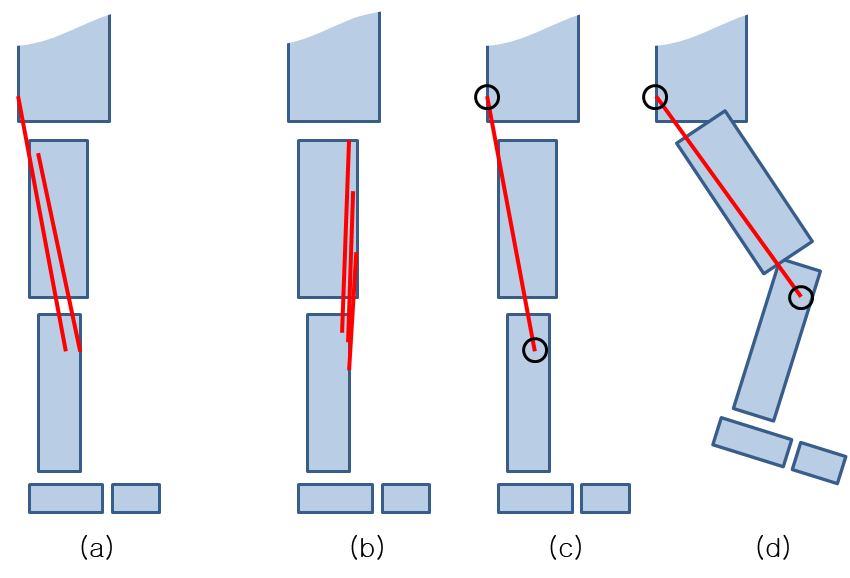
\includegraphics[width=3.5in]{muscleabs}
  \caption[Musculoskeletal modeling of a biped]{Musculoskeletal modeling of a biped:
  Black circles on (c) and (d) denote ball joints connecting both ends of the muscle to bones.}
  \label{muscleabs}
\end{figure}


%Our character model is a full four-limbed biped, which consists of 14 rigid bodies.
%The list of rigid bodies with their configurations is given in Table \ref{bipedconf}.

%Mass of each body segment is referenced from \cite{humanbodydynamics}.
%We assume a uniform mass distribution for each rigid body.
%Length of each body is calculated from the skeleton configuration of motion capture data~\cite{cmumocap}.
%Other dimension is chosen arbitrarily.

%\begin{table}[h!]
%\centering
%  \begin{tabular}{crrl}
%                                                         & Name      & Mass $(kg)$  & Dimension $(m \times m \times m)$  \\
%  \hline
%  \multirow{8}{*}{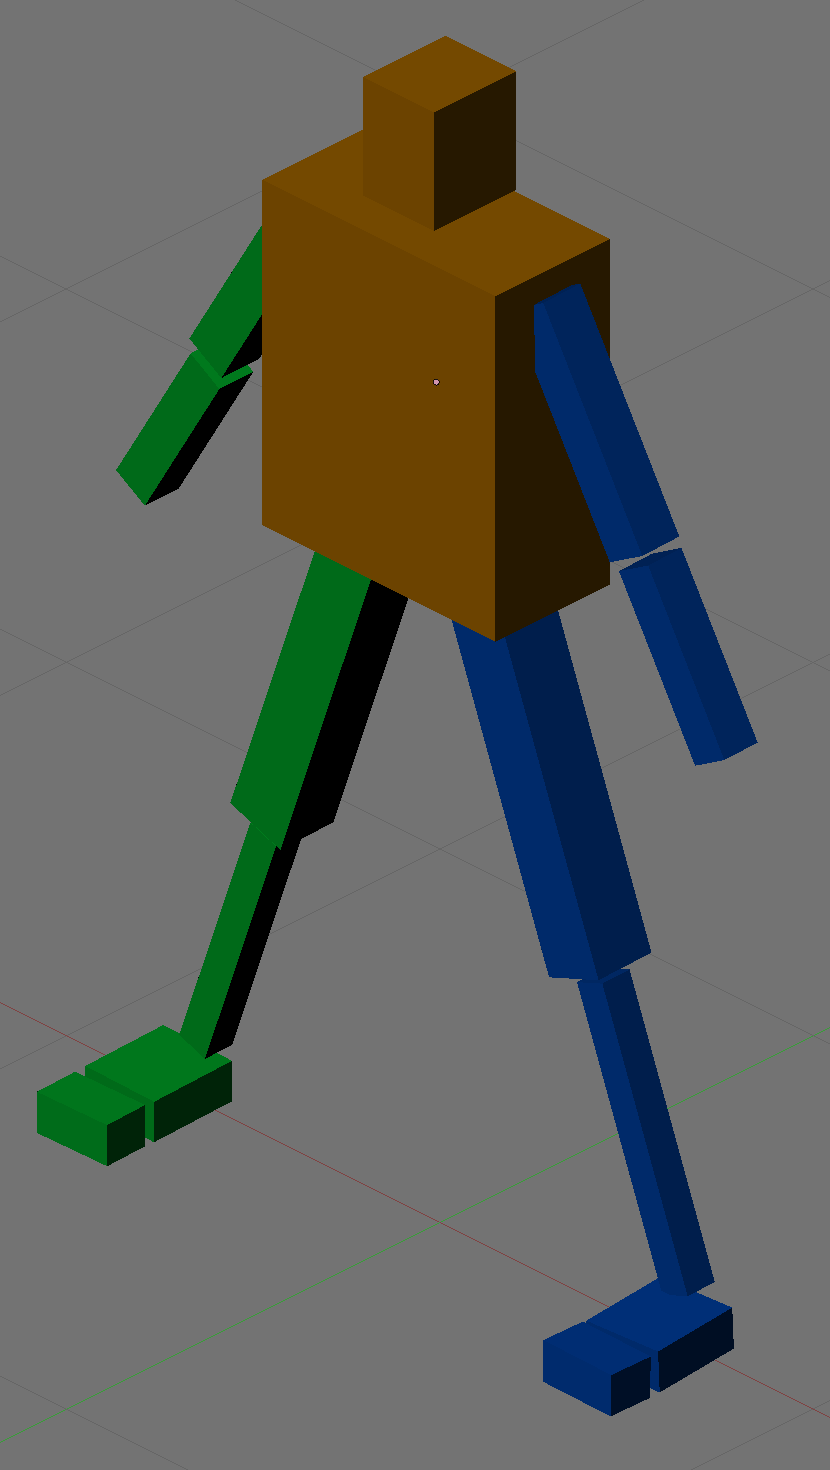
\includegraphics[width=0.85in]{biped}} & head      & 4.3          & $0.190 \times 0.220 \times 0.180$  \\
%                                                         & trunk     & 29.0         & $0.623 \times 0.507 \times 0.307$  \\
%                                                         & calf      & 2.7          & $0.073 \times 0.450 \times 0.073$  \\
%                                                         & thigh     & 6.3          & $0.142 \times 0.643 \times 0.142$  \\
%                                                         & sole      & 0.7          & $0.184 \times 0.210 \times 0.090$  \\
%                                                         & toe       & 0.2          & $0.184 \times 0.105 \times 0.090$  \\
%                                                         & upper arm & 2.0          & $0.100 \times 0.520 \times 0.100$  \\
%                                                         & lower arm & 1.1          & $0.090 \times 0.400 \times 0.090$  \\
%  \hline
%\end{tabular}
%\caption{Biped configuration}
%\label{bipedconf}
%\end{table}


\section{Muscle fiber model}

There are various muscle fiber models used in biomechanical field ranging
from a simple time-invariant spring model to a complicated time-varying model~\cite{25733}.
Although a more sophisticated model gives us a more realistic behavior, unnecessarily
complicated models will make the biped hard to simulate and control.
We use one of the simplest time-invariant spring-damper model commonly called
a Hill-type muscle model \cite{hill} as depicted in Figure \ref{hilltype}

\begin{figure}[h!]
  \centering
  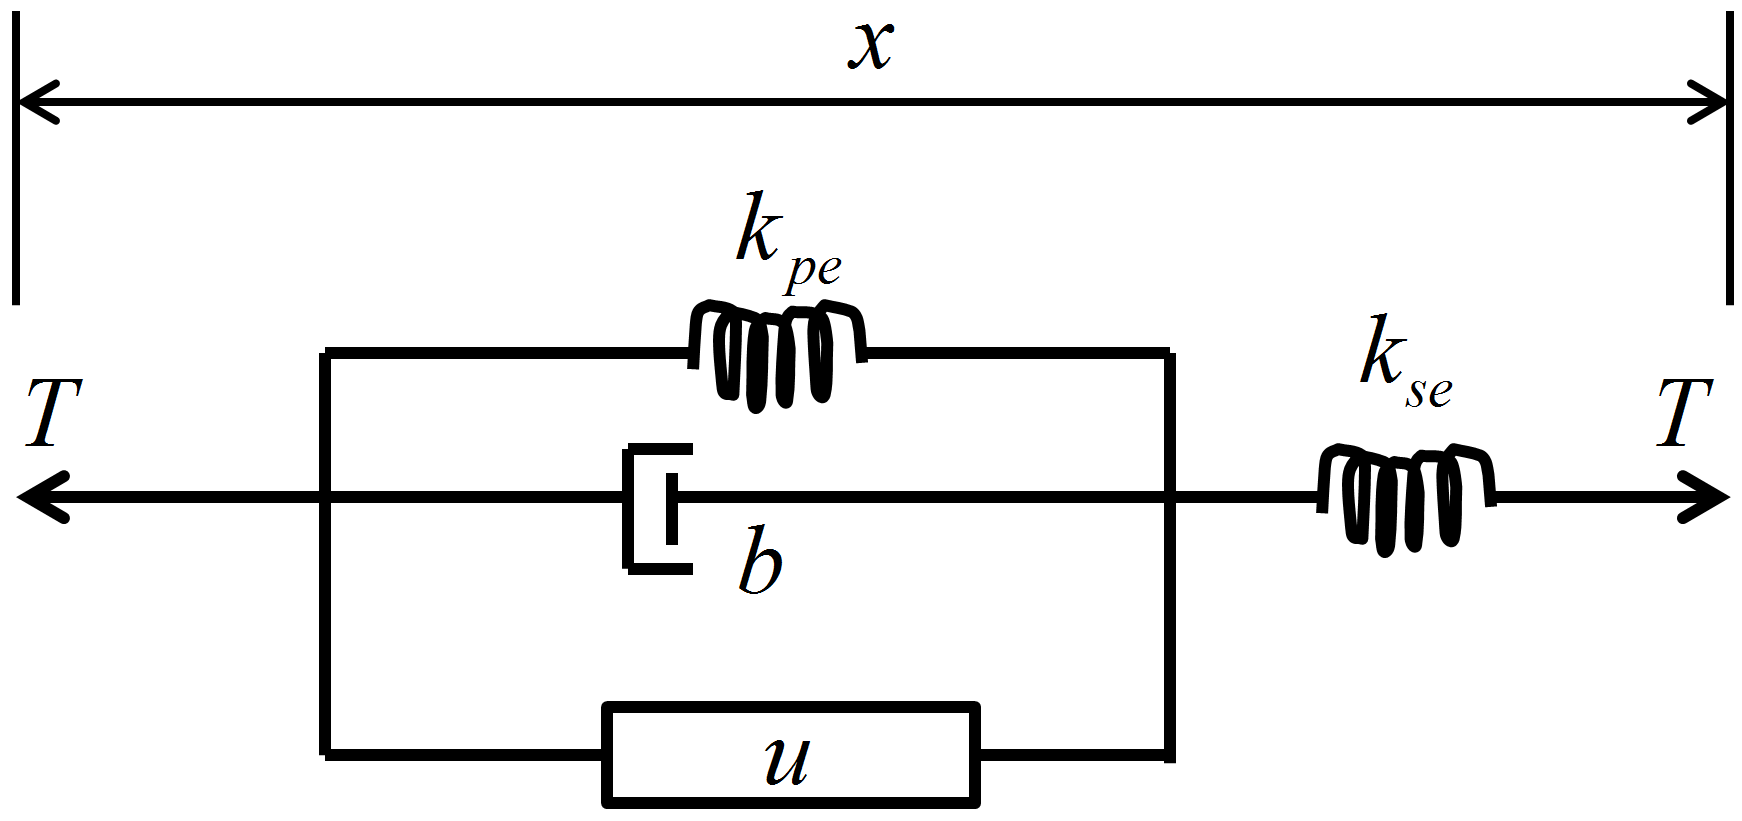
\includegraphics[width=2.6in]{musclemodel}
  \caption{Hill type muscle model}
  \label{hilltype}
\end{figure}
\noindent Basically, the model consists of two springs, a viscous damper and an uniaxial actuation component.
The damper and one of the springs are connected in parallel and the other spring is
connected in serial.
In real human body, many muscle fibers form fascicles, and multiple fascicles form a muscle body.
To simplify our biped model, we model a muscle body as a set of muscle fibers.
In the Hill-type muscle model, we need four parameters:
a serial spring constant $k_{se}$, a parallel spring constant $k_{pe}$, a viscosity $b$ and a rest length $x_{r}$.
These parameters can be constants or variables depending on how muscle fibers modeled.
A mathematical expression defining the dynamics of a muscle fiber is a first-order ordinary differential equation:
\begin{equation}\label{Tension}
\dot{T} = \frac{k_{se}}{b} \left( k_{pe}(x-x_{r})+b\dot{x}-\left(1+\frac{k_{pe}}{k_{se}}\right)T+u   \right)
\end{equation}
where $T$ is a tension exerted at both ends (positive means pulling),
$x$ is the length of the fiber and $u$ is actuation force in the active component.
Note that all quantities shown in the equation are scalar values.
Each muscle fiber always connects two different rigid bodies and the same amount of
tension is applied to both of them in the opposite directions.

Equation \eqref{Tension} can be transformed to a discretized version as done in equations of motion \eqref{MoEq2}.
Therefore, $T^{(l+1)}$ can be expressed as a linear function of $T^{(l)}$, $x^{(l+1)}$, and so forth.

We use muscle terminologies to clearly define the configuration of muscles.
A muscle fiber has an $origin$ and an $insertion$ which indicate the attached positions
of various muscle fibers at certain bones.
In other words, an origin and an insertion are used to indicate where a muscle fiber is originated from and inserted to, respectively.
If we denote the origin and the insertion positions of the fiber as $p_{org}$ and $p_{ins}$ defined in
the local Cartesian coordinates of respective bodies,
the normalized direction of the fiber is specified by
$\hat{d}^{W}=(p^{W}_{ins}-p^{W}_{org})/||p^{W}_{ins}-p^{W}_{org}||$ where
the superscript $W$ means that the positions are defined in the world coordinates.
Thus, we can calculate tensions $T\hat{d}^{W}$ and $-T\hat{d}^{W}$.
These two forces are applied to the origin and the insertion positions of the fiber, respectively (Figure \ref{orgins}).

\begin{figure}[h!]
  \centering
  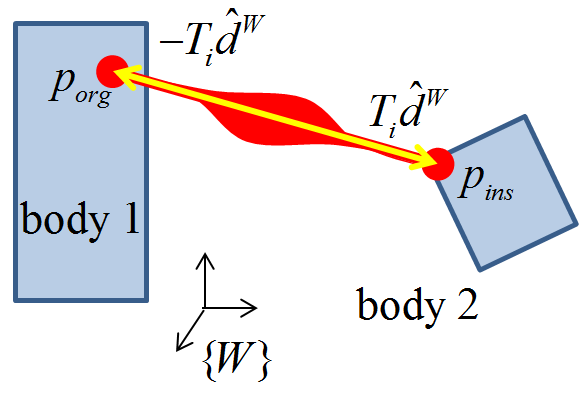
\includegraphics[width=1.8in]{orgins}
  \caption{Configuration of a muscle fiber attached to two rigid bodies}
  \label{orgins}
\end{figure}

We use two types of muscle fibers: actuated and unactuated muscle fibers.
Actuated muscle fibers represent the muscles that can be actuated voluntarily.
In fact, most of skeletal muscles are voluntary muscles.
On the other hand, unactuated muscle fibers are nonvoluntary and represent
ligaments of human body.
Typically they are attached around joints and keep joints connected.
Their purpose is to maintain its rest length to prevent joint dislocation.
For this reason, serial spring constants $k_{se}$ for unactuated fibers (ligaments)
are comparatively larger than those of the actuated muscle fibers.

%An \emph{agonist}, or \emph{prime mover}, is a muscle whose contraction is chiefly responsible for producing a particular movement.
%A muscle fibers has its \emph{antagonist}. The antagonist is a muscle whose action opposes that of a particular agonist.
%We can choose specific muscle fibers to be used in the biped model based on agonists related to legs.
%Also we can inform the optimizer to reduce actuation force on a muscle fiber when its antagonist is actively actuated.

\section{Soft joints}

Conventional biped models use reduced coordinates to represent a pose
because DOFs on rigid bodies can be reduced by connecting them with
joints. They use 6-DOF on the root of the biped, that is the pelvis for representing its position and orientation.
The other rigid bodies except the root have three or less DOFs depending on joint types and
typically have only the orientational freedom.
This implies that joint dislocation is not allowed with
conventional biped models.

On the contrary, every body segment of our biped model has a full 6-DOF
to allow joint dislocation.
From the dynamics point of view, multiple rigid bodies could be simulated individually
without any joint constraints involved.
Without joint constraints, the shape of biped figure would not be not maintained well
due to serious joint dislocation during optimization.
For instance, all body segments may collapse to the ground with their joints broken apart
convincing human poses can be maintained by limiting the degrees of joint dislocation.

We introduce soft joints which prevent serious joint dislocation on our biped model.
A soft joint is defined in terms of two points, $p_1$ and $p_2$, on the local coordinate systems of two
different rigid body segments, respectively as well as a dislocation threshold $r$ (Figure~\ref{fig:softjoint}).
Specifically, the distance between two points are constrained within $r$.
We connect two points with a stiff unactuated muscle fiber which helps satisfy the constraint.
Since $r$ is a small value, the unactuated muscle fiber length $||p_{1}-p_{2}||$ may becomes zero
or near zero during simulation. Thus, the normalized muscle fiber direction $d^W$ is not well-defined in this case.
We use an arbitrary $d^W$ whose norm is 1 to address this issue. This case arises only on unactuated fibers on soft joints.


%With these kind of joints, the biped can take advantages of shock absorption
%mechanism as well as prevention of joint dislocation.

\begin{figure}[h!]
  \centering
  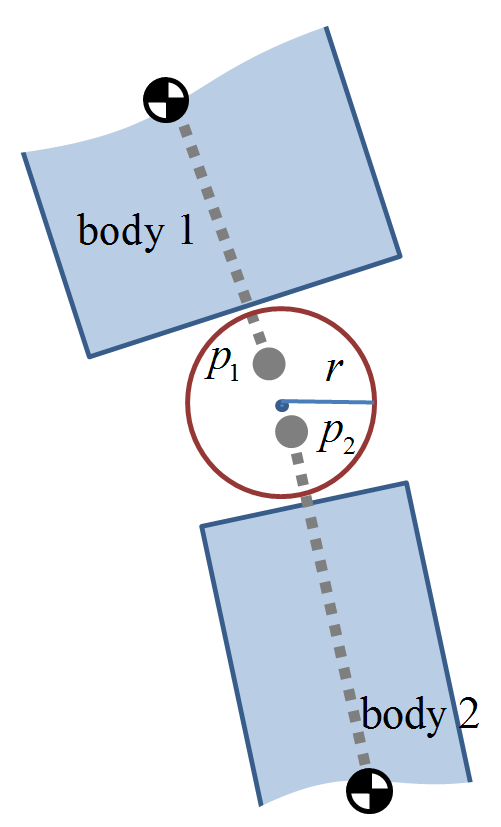
\includegraphics[width=1.3in]{softjoint}
  \caption{Structure of a soft joint}
  \label{fig:softjoint}
\end{figure}


\chapter{Physics simulation and optimization}

\section{Equations of motion}

Equations of motion governing the movement of rigid bodies can be written as follows:
\begin{equation}\label{MoEq2}
\mathbf{M}(\chi)\ddot\chi + C(\chi,\dot\chi )
 = f_g + f_c + f_f  + f_{ext} = f
\end{equation}
where $\mathbf{M}$ is a generalized mass matrix and $\chi$ is a generalized
linear and angular position
state vector, $\dot\chi$ and $\ddot\chi$ are its first and second time derivatives,
respectively. $C$ represents Coriolis and centrifugal forces.
$f_c$ represents contact forces or ground reaction forces.
$f_f$ denotes muscle forces due to muscle fiber tensions.

For a freely moving single
rigid body with 6-DOF with $n_f$ muscle fibers attached,
$\mathbf{M}$ will be $6\times 6$ matrix and $\chi$,
$C$, $f_g$, $f_c$ and $f_f$ will be a 6-dimensional vector. $f_f$ is the sum of
muscle forces, that is $\sum f_{f,i}$ where $i=1,\dots,n_f$.

Because we represent time as discrete samples, all the functions of
time-varying variables need to be represented in a discrete domain.
We discretize the time into samples with small intervals $h$. Accordingly,
the velocity $\dot\chi$ and the acceleration $\ddot\chi$ at current
time sample $l$ are defined by backward and central finite differences, respectively,
as follows:
\begin{align}
\dot\chi  \equiv {} & \frac{\chi^{(l)}-\chi^{(l-1)}}{h}\label{vel-dis},\\
\ddot\chi \equiv {} & \frac{\chi^{(l+1)}-2\chi^{(l)}+\chi^{(l-1)}}{h^2}.\label{acc-dis}
\end{align}
By substituting \eqref{vel-dis} and \eqref{acc-dis} into \eqref{MoEq2},
we can express $\chi^{(l+1)}$ as a linear function of $\chi^{(l)}$, $\chi^{(l-1)}$ and so forth.
Notice that we embedded Euler integration step into the equations of motion by this substitution.

As stated in Chapter 1, most of the existing work on
character animation used an articulated body to represent a character.
In the articulated model, each body is connected to another body with
various types of joints such as hinge joints and ball joints.
Therefore, so-called joint constraint equations are additionally
needed for that model.
On the other hand, since we use no joint at all in the character
model, the equations of motion of the whole biped is just a independent collection of
\eqref{MoEq2}. Thus, we have the following matrix equation

\begin{equation}
\left [
\begin{array}{ccc}
\mathbf{M}_1                      &            &                               \\
                                  &  \ddots    &                               \\
                                  &            & \mathbf{M}_{|\mathcal{B}|}    \\
\end{array}
\right ]
\left [
\begin{array}{c}
\ddot{\chi}_1 \\
\vdots \\
\ddot{\chi}_{|\mathcal{B}|}
\end{array}
\right ]
+
\left [
\begin{array}{c}
C_1 \\
\vdots \\
C_{|\mathcal{B}|}
\end{array}
\right ]
=
\left [
\begin{array}{c}
f_1 \\
\vdots \\
f_{|\mathcal{B}|}
\end{array}
\right ]
\end{equation}
where $\mathcal{B}$ is a set of body segments constituting the biped.
Since this permits independent rigid body movements,
our model may allow joint dislocation.
We will use soft joint constraints to prevent serious
joint dislocation in the subsequent section.



\section{Contact model}
\label{sec:contact}

We use a penalty-based method which can be integrated easily in our optimization framework.
It estimates contact normal forces by allowing a certain amount of penetration between a pair of bodies.
A temporary spring-damper element is created and attached where a contact is established.
The spring-damper exerts a strong force to separate the two penetrated bodies.
After the non-penetration constraints recovered the spring-damper element is removed immediately.
Typically, a critically-damped spring is used to minimize the separation time minimal without oscillation.

\begin{figure}[h!]
  \centering
  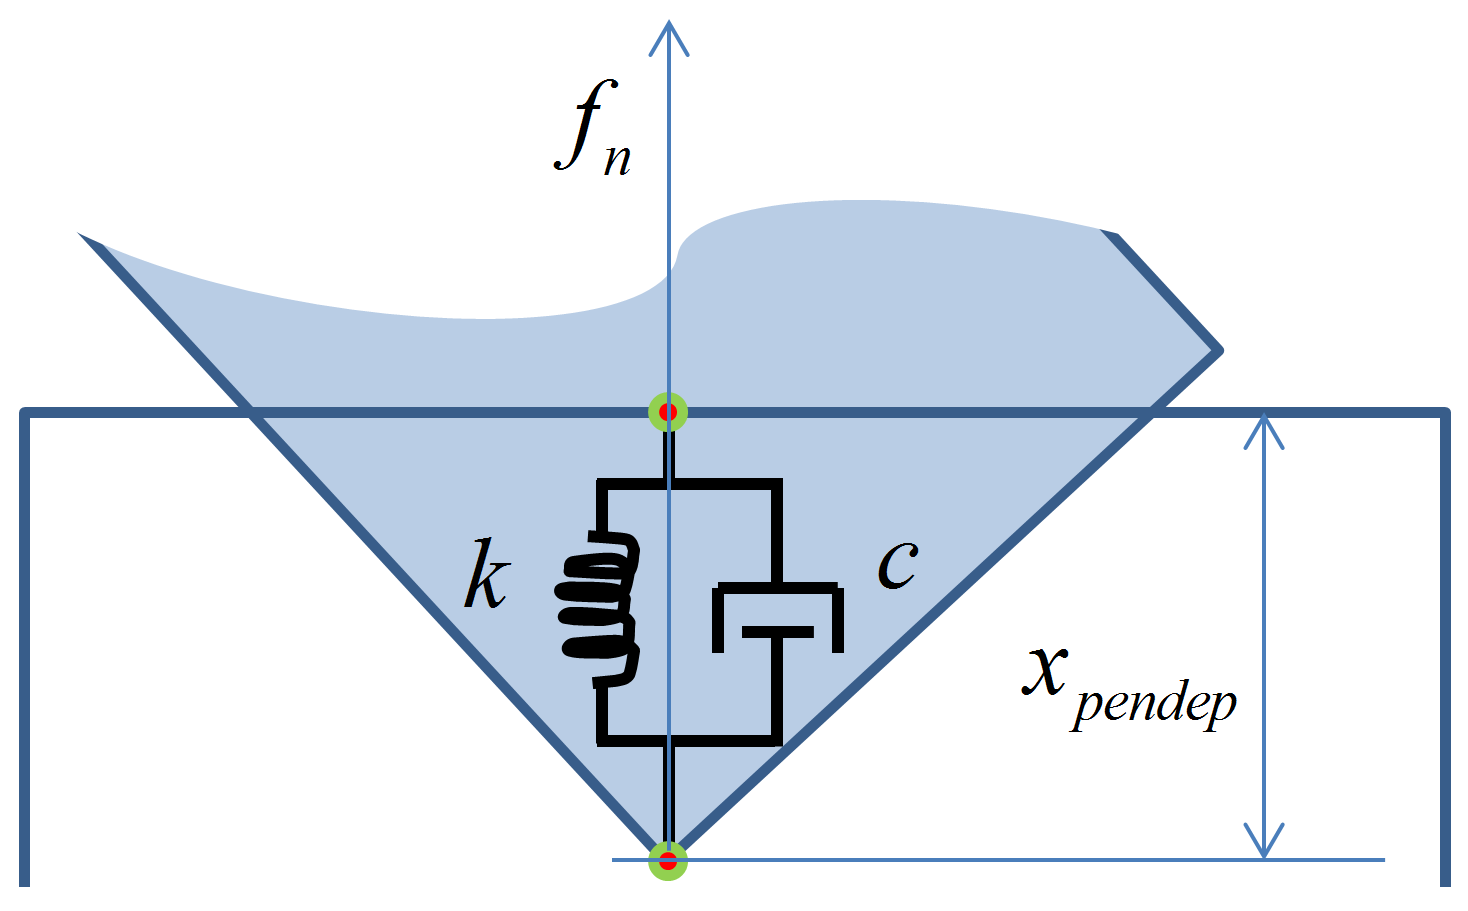
\includegraphics[width=2.0in]{penalty}
  \caption{Normal force calculated from the penalty method}
\end{figure}

The normal force exerted at the penetrated corner point of the box is calculated as follows:
\begin{equation}\label{penalty-normal}
f_n = -k x - c \dot{x}
\end{equation}
where $f_n$ is the normal force, $k$ is a spring constant, $c$ is a damping coefficient and $x$ is
a penetration depth. $k$ and $c$ is positive numbers and $x$ is a negative in case of penetration.
If a single rigid body of body mass $\bar{m}$ has $n_p$ contact points with the ground,
$n_p$ springs of the damping coefficient $c=2\sqrt{\bar{m}k/n_p}$ makes a critically damped system.

Since any normal force should be applied in a unilateral manner, that is
only pushing a penetrated body but not pulling it, we need an additional constraint $f_n \geq 0$.
$x$ is always negative, so that the term $-kx$ always becomes positive.
A problem arises at a penetrated corner point in a separation phase;
especially when $-kx < c\dot{x}$ which leads $f_n$ to a negative value.
To circumvent this issue, we add a nonnegative positive scalar term $\lambda$ to the right-hand side
of Equation~\eqref{penalty-normal}.
A minimal $\lambda$ is computed to satisfy the constraint in optimization by setting
a very high cost on $\lambda$. We further discretize the resulting constraint to obtain

%obey the constraint $f_n \geq 0$. During optimization,
%a minimal $\lambda$ to keep the constraint will be calculated
%when we set a very high cost on that variable. We can denote \eqref{penalty-normal} with
%discrete-time substitution that can be used as an equality constraint for the optimizer.

\begin{equation}\label{penalty-normal-discretized}
f_n = -k x^{(l+1)} - c \frac{x^{(l+1)} - x^{(l)}}{h} + \lambda.
\end{equation}
Besides the normal force, the tangential contact force is needed to model friction.
We employ the Coulomb friction model to do it.
There are two kinds of friction in this model: static friction and dynamic friction.
If contact points are sliding along the surface without breaking contacts,
dynamic friction forces will act upon them. In this case, the friction force is depends
on the magnitude of the normal force of a sliding contact point and its velocity along the surface.
Dynamic friction force $f_{tk}$ is
\begin{equation}\label{dynamic-friction}
f_{tk} = -\mu_k v ||f_n||
\end{equation}
where $\mu_k$ is a coefficient of dynamic friction
and $v$ is the velocity of a sliding contact point along the surface.
On the other hand, a static friction force is generated at a stationary contact point.
In this case, a contact force lies on a cone-shaped region so-called
the Coulomb's friction cone. It is allowed to choose any static friction force as far as
the resulting contact force is in the cone.
The conditions for the static friction force can be expressed as follows:
\begin{equation}\label{static-friction}
\mu_s ||f_n|| \geq ||f_{ts}||, \quad f_{ts} \cdot \hat{f}_n = 0
\end{equation}
where $f_{ts}$ is the static friction force and $\mu_s$ is the coefficient of static friction.
The inner product equality implies that $f_{ts}$ lies on the tangential space of contact point.



\section{Optimization}
In this section, we design a tracking controller based on an optimization technique.
Given our biomechanical biped model as well as basic building blocks defined in the previous
sections for rigid body dynamics simulation.
There are four types of constraints: equations of motion, muscle fiber tensions, contact forces and soft joints.
Equations of motion (Equation~\eqref{MoEq2}) govern motions of rigid bodies composing the biped.
Muscle fiber tensions cannot be chosen arbitrarily but should be calculated from the
discretized version of Equation~\eqref{Tension}
which is a linear function of actuation forces $u$, muscle fiber length $x$ and its rest length $x_r$.
Contact forces conform Equations \eqref{penalty-normal-discretized} and \eqref{static-friction} if
they are static; otherwise they conform Equations \eqref{penalty-normal-discretized} and \eqref{dynamic-friction}.
Lastly, soft joint constraints prevent serious joint dislocation.

\begin{equation}\notag
\text{minimize} \quad w_{ref} || \chi^{(l+1)} - \bar{\chi}^{(l+1)} || + w_u || u ||
\end{equation}
\begin{align}
\text{subject to} & \quad \chi^{(l+1)} = \tilde{\mathbf{M}}^{-1} (f_g + f_c + f_f + f_{ext} - \tilde{C})     &                      \label{moeq-dis}\\
                  & \quad f_{f,i} = (-1)^{q} ( A_i u_i + B_i x_r + C_i ) d^W_i                               & i \in \mathcal{M}    \label{mf}\\
                  & \quad f_{c,i} = f_{n,i} + f_{tk, i}                                                      & i \in \mathcal{P}_k  \notag\\
                  & \quad f_{c,i} = f_{n,i} + f_{ts, i}                                                      & i \in \mathcal{P}_s  \notag\\
                  & \quad r_i \geq || Z_i \chi^{(l+1)} + V_i ||                                              & i \in \mathcal{J}    \label{sj}\\
                  & \quad u_{min}   \leq u   \leq u_{max}                                                    &                      \notag\\
                  & \quad x_{r,min} \leq x_r \leq x_{r,max}                                                  &                      \notag\\
                  & \quad f_{f,min} \leq f_f \leq f_{f,max}                                                  & i \in \mathcal{M}    \notag
\end{align}
A variable $q$ in Equation~\eqref{mf} is 0 or 1
if tension is acting on the origin body. Otherwise, it is 1.
$\mathcal{P}_k$ and $\mathcal{P}_s$ denote a set of dynamic contacts and a set of static contacts, respectively.
Note that we omit some constraints such as the Coulomb friction cone constraints (Equation~\eqref{static-friction}) for brevity.
In Equation \eqref{sj}, we estimate the next step's joint anchor position in the world coordinate frame.
We refer the readers to \cite{Jain:09:OIM} for detailed derivation.

The optimizer tries to find next pose $\chi^{(l+1)}$ which is as close as possible
to $\bar{\chi}^{(l+1)}$ with minimal efforts.
Optimization variables are $u$, $x_r$ and $f_{ts}$.
Solving the optimization problem is done at each simulation frame.
After next pose $\chi^{(l+1)}$ is calculated, the current pose is updated
and the frame counter $l$ is increased by 1.




\chapter{Results}

We implemented the biomechanical biped simulator, and experimented
it on various locomotion reference motions.
As an optimization solver, we used the MOSEK optimization software~\cite{mosek} to solve
the optimization problem presented in the previous chapter.
The experiments were done on Intel Core 2 Quad 2.66 GHz processor and 8 GB of RAM.
To show that our reference tracker follows given reference motion well,
we measured the deviation error $\epsilon^{(l)}=||\chi^{(l)}-\bar{\chi}^{(l)}||$
between the reference and simulated poses at each frame.

As reference trajectories $\bar{\chi}$, we used Carnegie Mellon
University's Graphics Lab Motion capture database~\cite{cmumocap}.
Specifically, we used five motion clips from 07\_01 to 07\_05
in the category `Locomotion/Walking'.
In order to establish contact points in a stable manner,
we modified foot and sole trajectories to properly align with
the ground floor in stance phase.
Since the original motion clips are sampled in 120 Hz, we resampled
the reference data using the B\'{e}zier curve interpolation
in accordance with the simulation time interval $h$.

The friction coefficient $\mu$ for static and dynamic contacts was set to 1.0.
$k=5000$ $Nm^{-1}$ was used for the ground spring constant and
the simulation time step interval is chosen as $h=0.002$ second.
There are a large number of parameters to be preset for muscle fibers.
We used parameters provided in OpenSim~\cite{Delp07}.
Although the Schutte muscle model was used in it instead of our Hill-type muscle model,
two models share similarity in their sub-elements.
Since OpenSim does not provide parameters for ligaments, we arbitrarily
chose ligament parameters using $k_{se} = 1000~Nm^{-1}$, $k_{pe} = 0$ and $b=0.1~Nms^{-1}$
on our soft joints. Joint dislocation threshold $r$ was set to $0.03~m$.

\begin{table}[h!]
\centering
  \begin{tabular}{cccccc}
  motion clip                      &  type         & frames  & resampled frames & duration (s) & $\bar{\epsilon}$\\
  \hline
  07\_01                           &  walk         & 315     & 1312             & 2.63     &     0.185           \\
  07\_02                           &  walk         & 329     & 1370             & 2.74     &     0.186           \\
  07\_03                           &  walk         & 415     & 1729             & 3.46     &     0.189           \\
  07\_04                           &  slow walk    & 450     & 1875             & 3.74     &     0.341           \\
  07\_05                           &  slow walk    & 517     & 2154             & 4.31     &     0.266           \\
  \hline
\end{tabular}
\caption{Statistics on reference tracking simulation}
\label{stat}
\end{table}

Characteristics on the reference data and tracking error are shown in Table~\ref{stat}.
$\bar{\epsilon}$ denotes the average difference over all frames, that is,
$\bar{\epsilon} = \sum_{i=1}^{n}\epsilon^{(l)}/n$ where $n$ is the number of
resampled frames. The snapshots of simulated motion for the motion clip 07\_01 were
shown in Figures \ref{fig:snapshot1} and \ref{fig:snapshot2},
where the green boxes and the red lines represent the rigid segments of the biped and
the reference motion, respectively.


%The difference between the reference trajectory and simulated motion for each
%frame is shown in Figure \ref{fig:devi}. The difference mainly arose
%because of soft joints. Since we allowed joints to dislocate at some range,
%the error resulted from whenever a foot contact occurred.

%The cost function of optimization plays a great role for tweaking
%animation. For instance, if we suppress the actuation force by increasing $w_u$
%the biped will move limply. Note that arbitrary
%weights do not always give the proper motion sequence.

Theoretically, if we set a joint dislocation threshold $r$ to 0, our
biped model becomes an articulated figure with rigid joints.
However, this would make our optimization formulation infeasible frequently
since the ligaments are not stiff enough to maintain zero dislocation of the joints.

Our biped model and simulated motions are physically valid since
we enforced equations of motion on all rigid segments
as equality constraints in the optimization formulation.
These constraints (Equation~\eqref{moeq-dis})
are physically correct up to discretization errors.
Besides, the contact model (Section~\ref{sec:contact}) is also consistent
except that it allows certain degrees of penetration.

The size of optimization problem is mainly
dependent on the number of rigid segments, muscle fibers, soft joints
and contact points. Except for contact points, all components
constituting the biped was the same for the whole simulation process.
Therefore, runtime performance varied between frames
with respect to the number of contact points. On average, the solver took
about 0.1 to 0.2 seconds per frame.



%Note that although we add an objective for minimizing the actuation
%forces on each actuated muscle fiber, this does not guarantee that
%actuation forces to be smooth.


%We used a straight walking motion sequence
%for a reference trajectory.

%Muscle fiber parameters can be varied to get different styles of motions.
%For example, a high $k_{se}$ gives more robot-like movement while a low value
%gives human-like elastic motion. However, viscous damping constant
%$b$ does not play a significant role in making various motions.

%Employing soft joints instead of rigid joints allows some limited
%dislocation. This leads to a better performance on tracking deviation.
%For example, let us assume that the biped extends its swing foot
%forward during tracking process. A contact time of swing foot with
%ground may differ from the reference trajectory
%and the simulated biped. By dislocating ankle, knee and hip joints
%a little, the contact time difference may be decreased.

%will affect every body segment because they are connected with
%one or more rigid joints. On the other hand, in our model,
%external force in a certain range on a body segment will only
%affect on that body by allowing a little dislocation on joints.

\begin{figure}
  \centering
  \subfloat{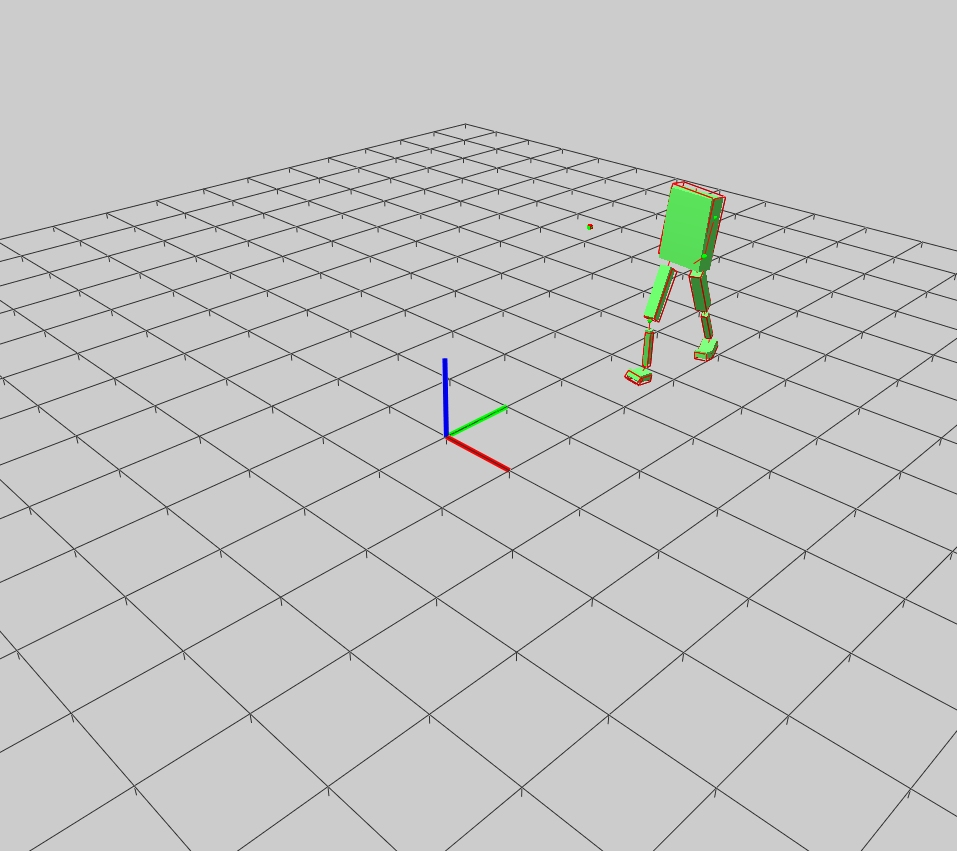
\includegraphics[trim = 70mm 80mm 70mm 50mm, clip, width=1.5in]{pymss/00001}}
  \subfloat{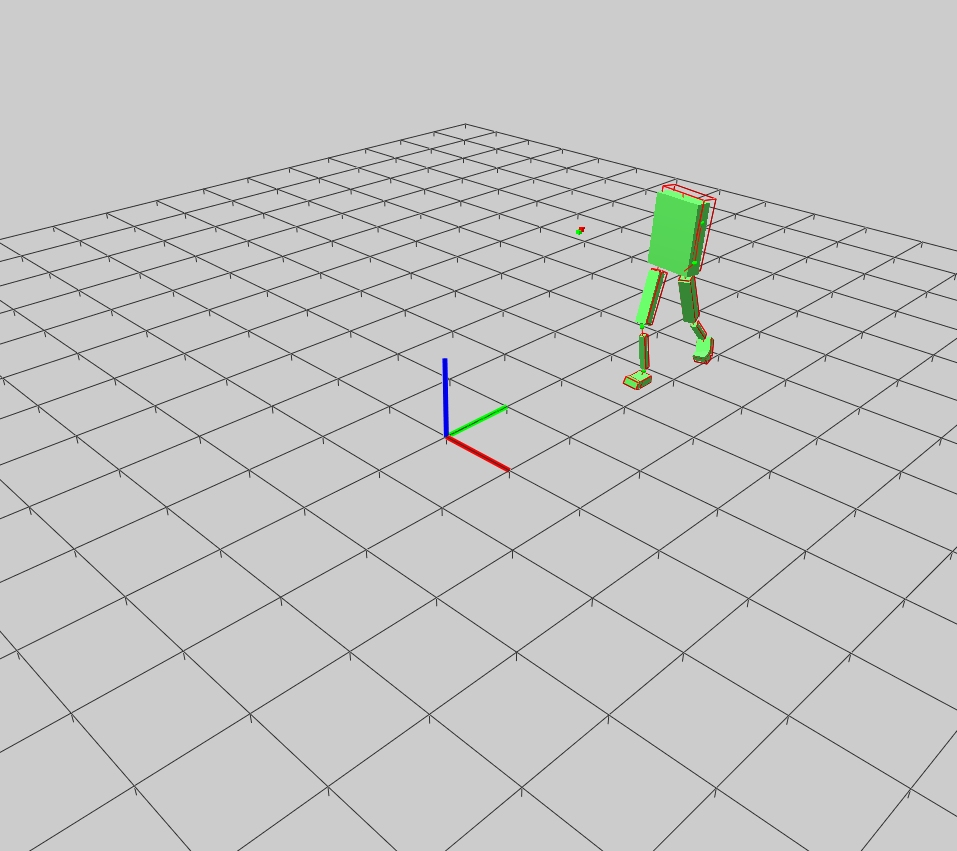
\includegraphics[trim = 70mm 80mm 70mm 50mm, clip, width=1.5in]{pymss/00031}}
  \subfloat{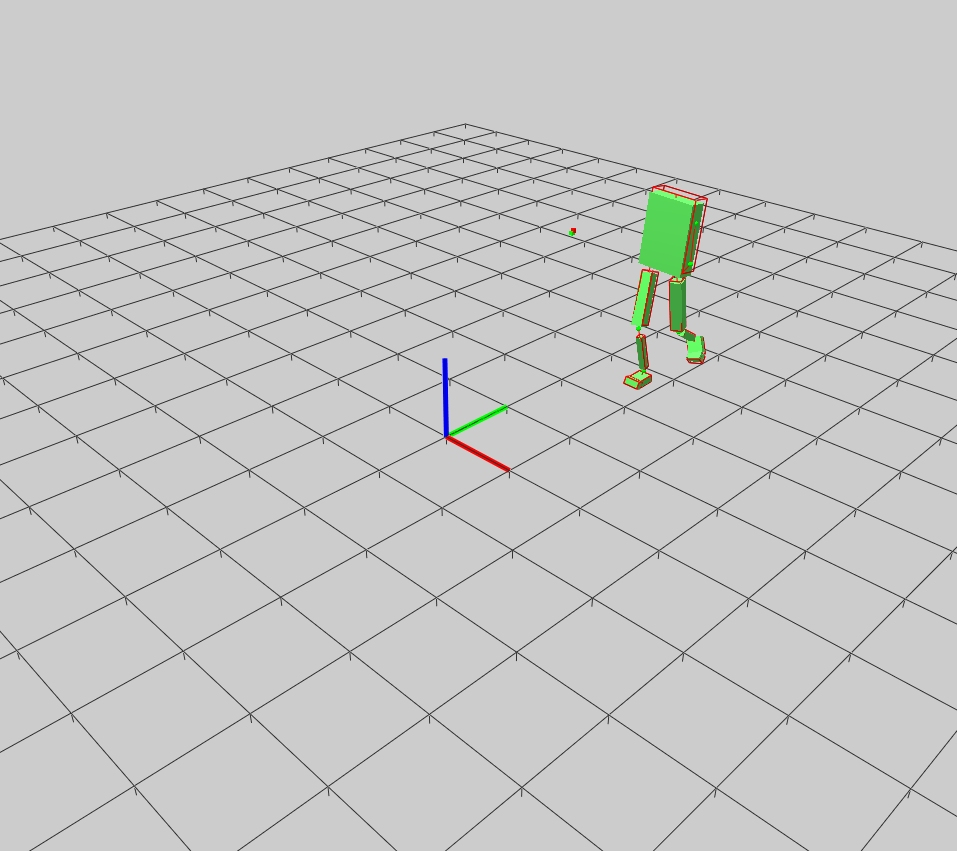
\includegraphics[trim = 70mm 80mm 70mm 50mm, clip, width=1.5in]{pymss/00061}}
  \subfloat{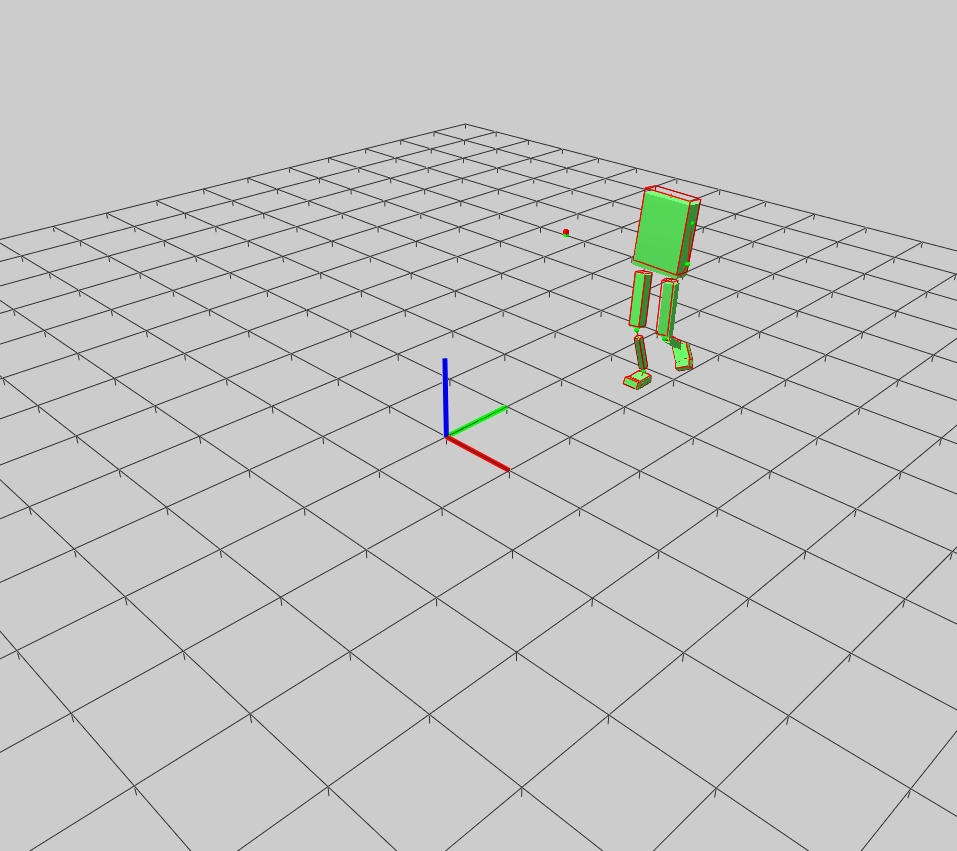
\includegraphics[trim = 70mm 80mm 70mm 50mm, clip, width=1.5in]{pymss/00091}}\\
  \subfloat{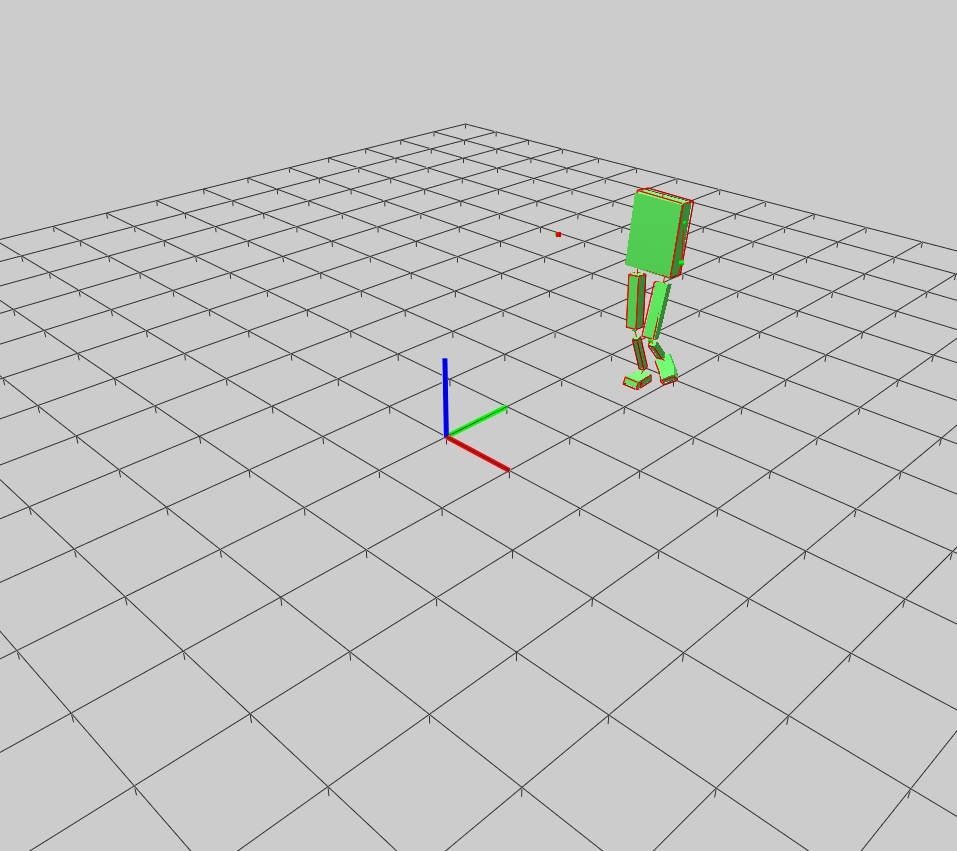
\includegraphics[trim = 70mm 80mm 70mm 50mm, clip, width=1.5in]{pymss/00121}}
  \subfloat{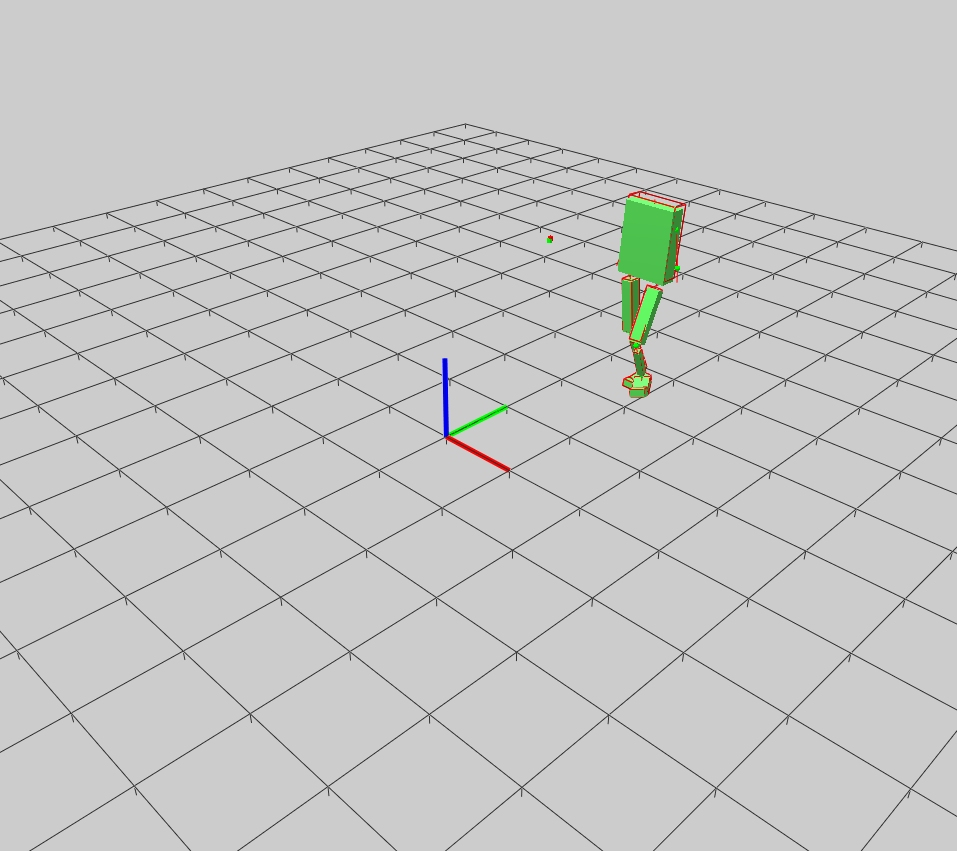
\includegraphics[trim = 70mm 80mm 70mm 50mm, clip, width=1.5in]{pymss/00151}}
  \subfloat{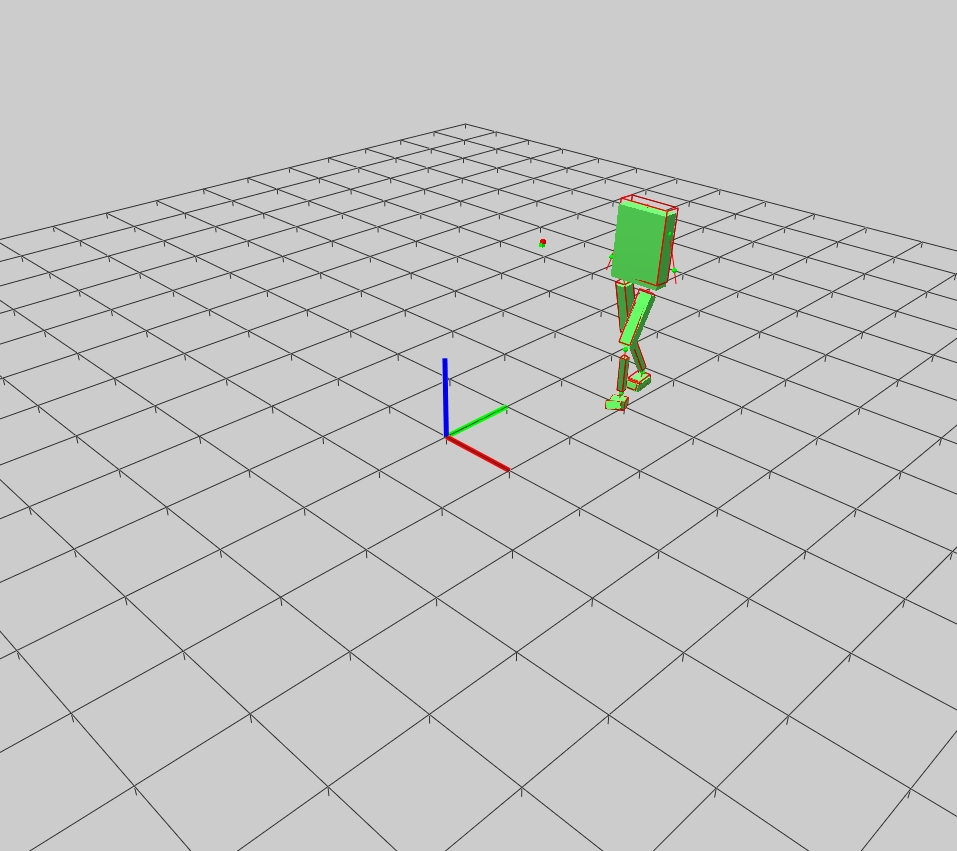
\includegraphics[trim = 70mm 80mm 70mm 50mm, clip, width=1.5in]{pymss/00181}}
  \subfloat{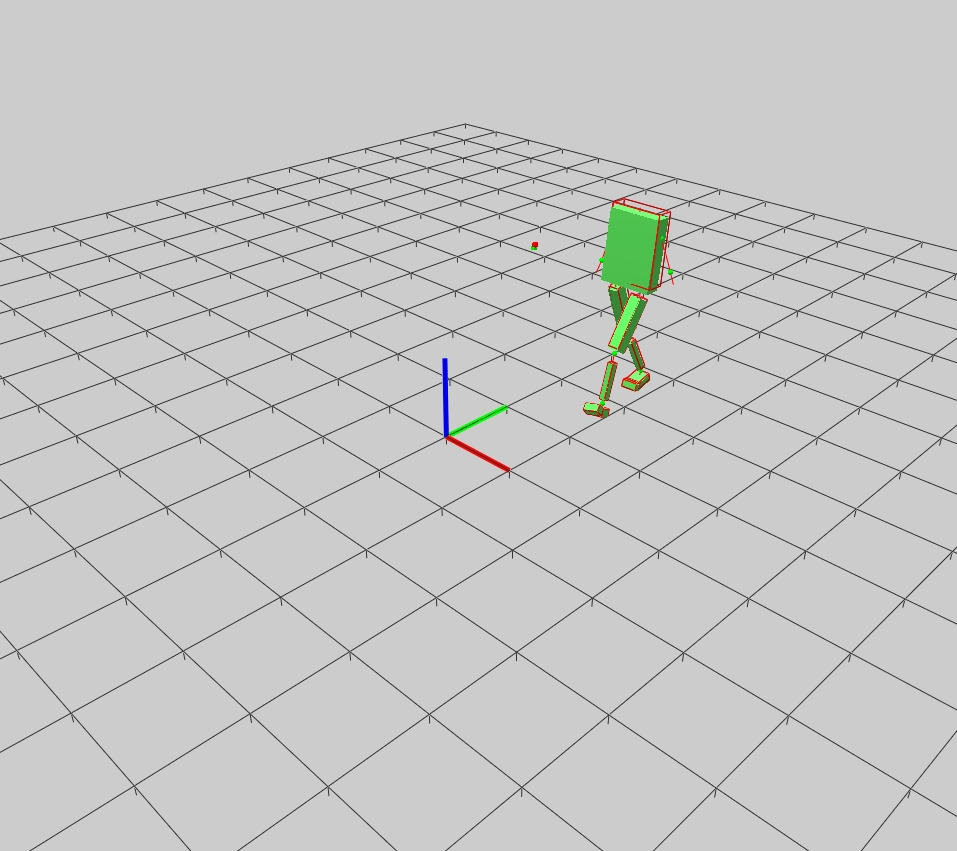
\includegraphics[trim = 70mm 80mm 70mm 50mm, clip, width=1.5in]{pymss/00211}}\\
  \subfloat{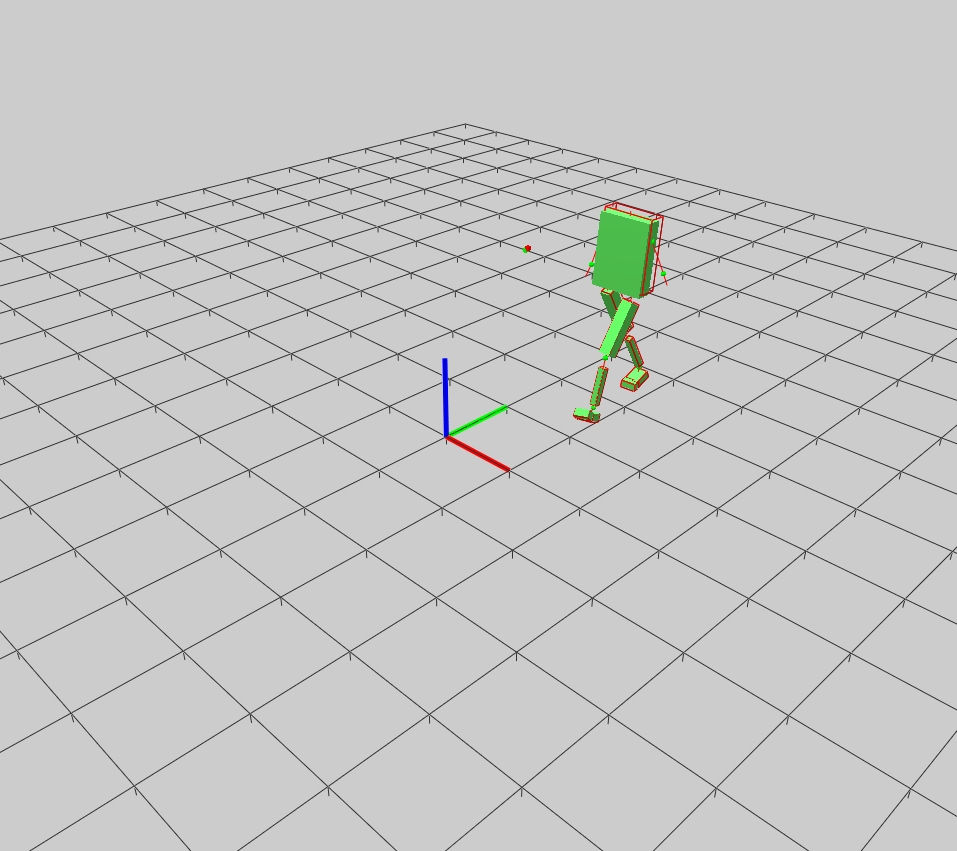
\includegraphics[trim = 70mm 80mm 70mm 50mm, clip, width=1.5in]{pymss/00241}}
  \subfloat{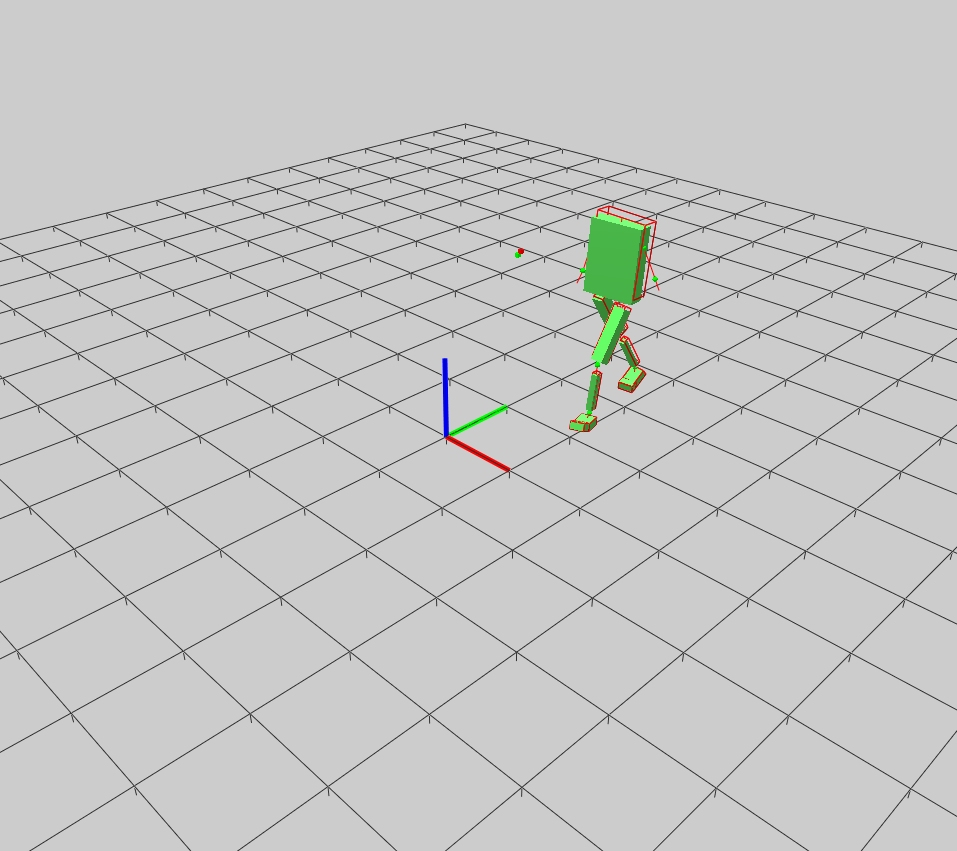
\includegraphics[trim = 70mm 80mm 70mm 50mm, clip, width=1.5in]{pymss/00271}}
  \subfloat{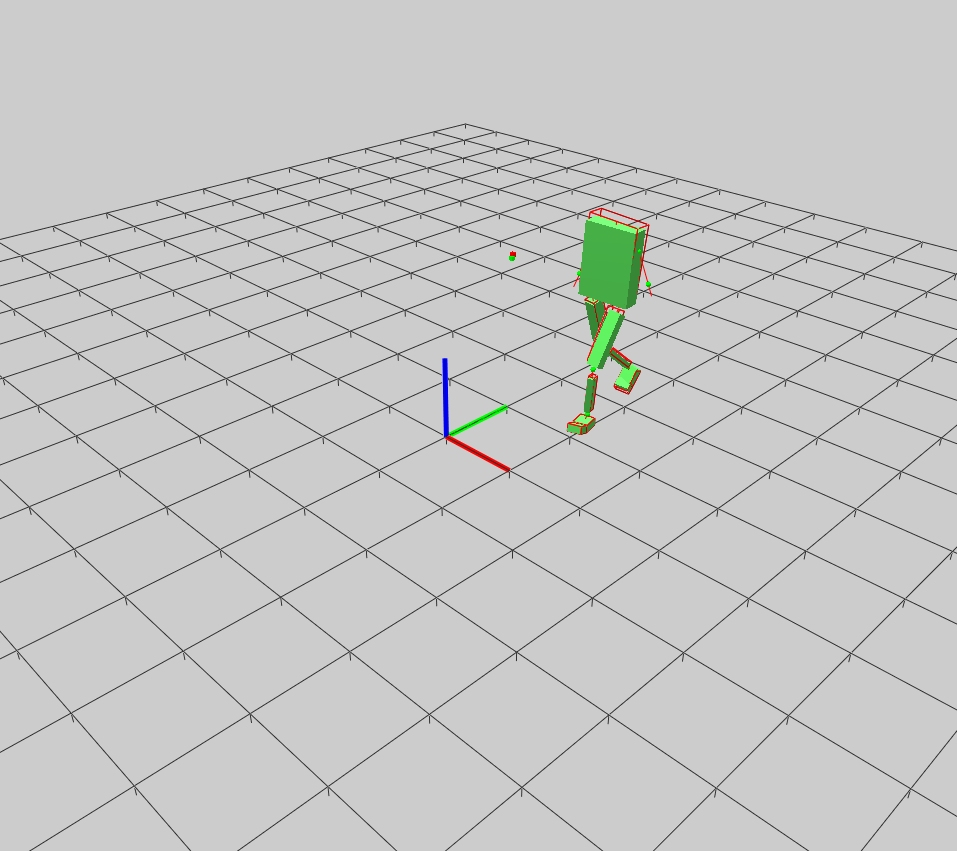
\includegraphics[trim = 70mm 80mm 70mm 50mm, clip, width=1.5in]{pymss/00301}}
  \subfloat{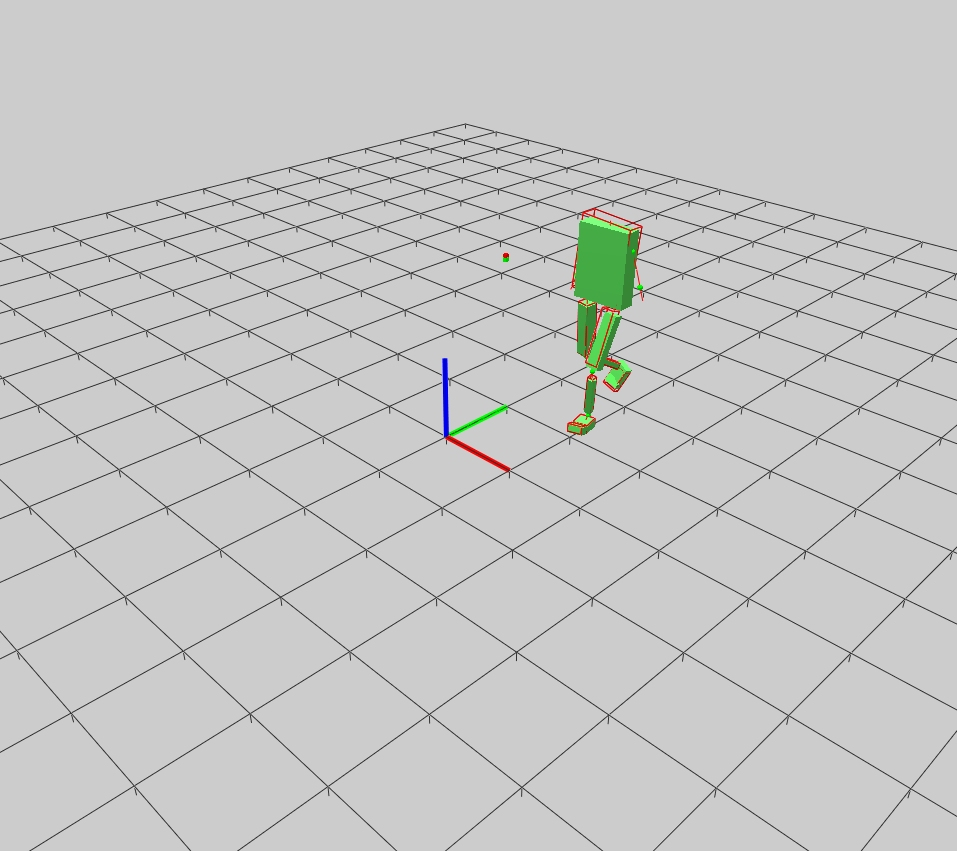
\includegraphics[trim = 70mm 80mm 70mm 50mm, clip, width=1.5in]{pymss/00331}}\\
  \subfloat{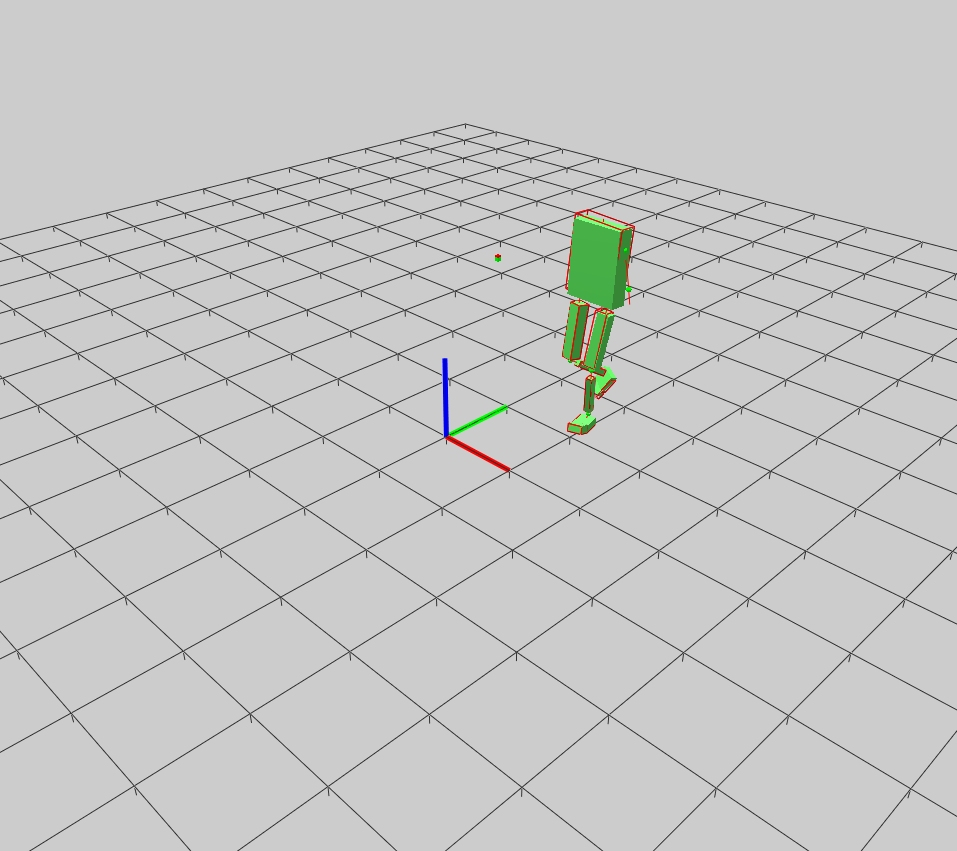
\includegraphics[trim = 70mm 80mm 70mm 50mm, clip, width=1.5in]{pymss/00361}}
  \subfloat{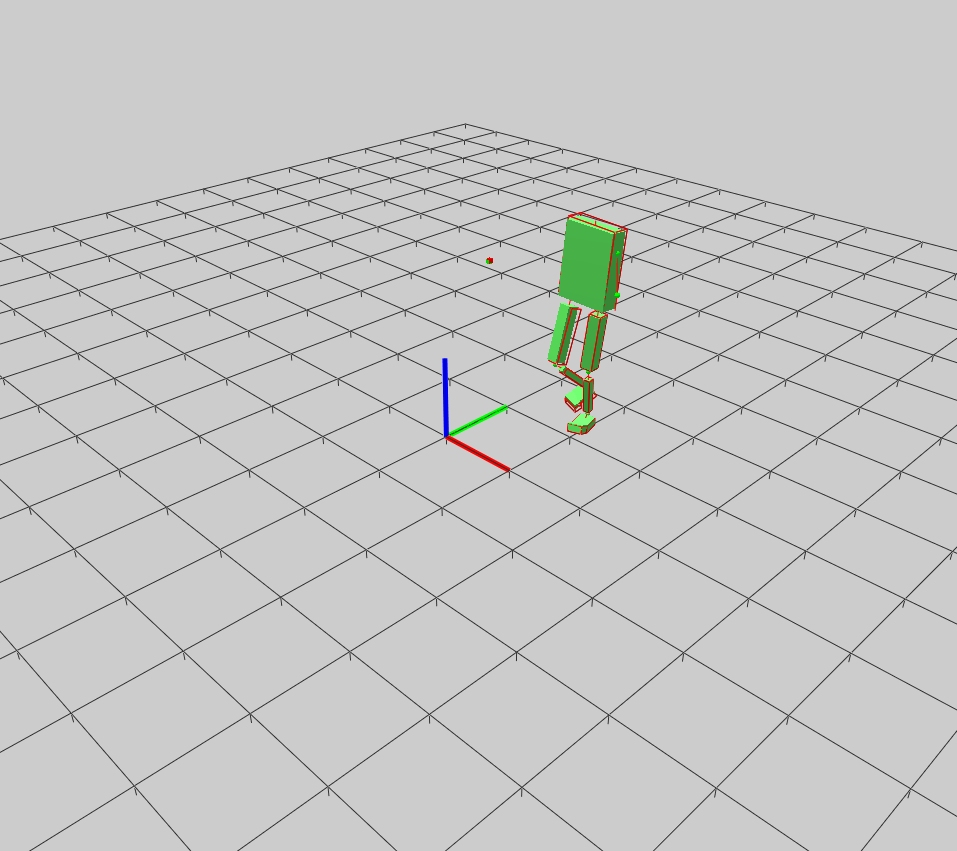
\includegraphics[trim = 70mm 80mm 70mm 50mm, clip, width=1.5in]{pymss/00391}}
  \subfloat{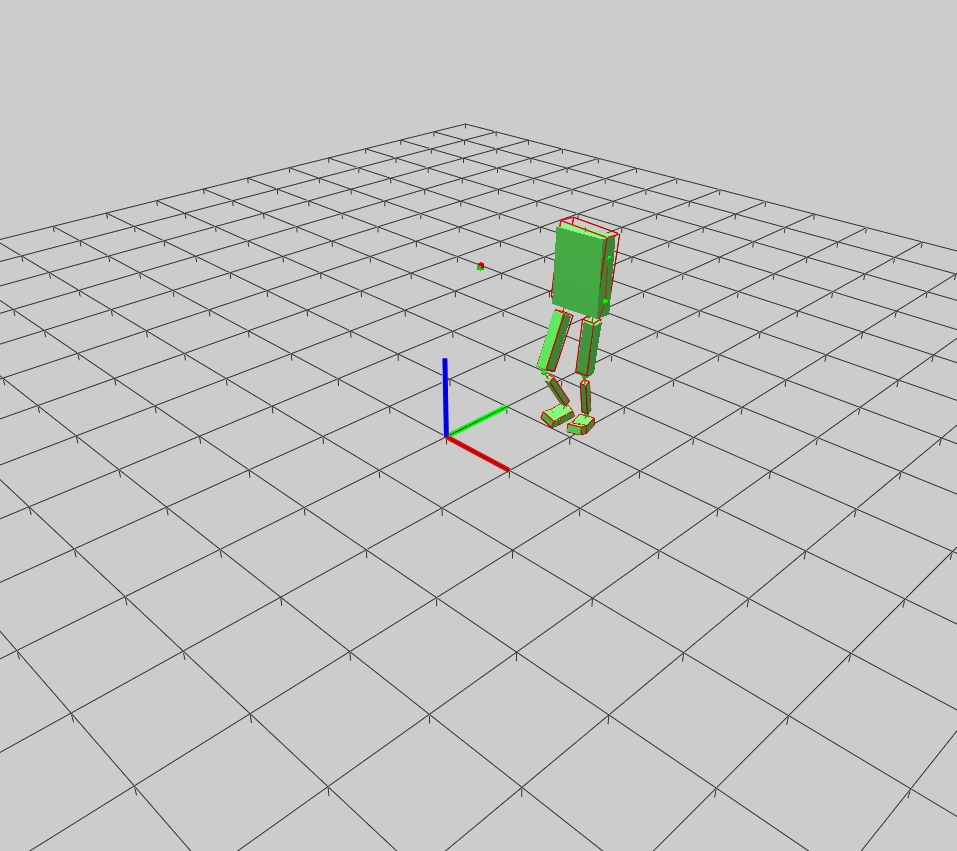
\includegraphics[trim = 70mm 80mm 70mm 50mm, clip, width=1.5in]{pymss/00421}}
  \subfloat{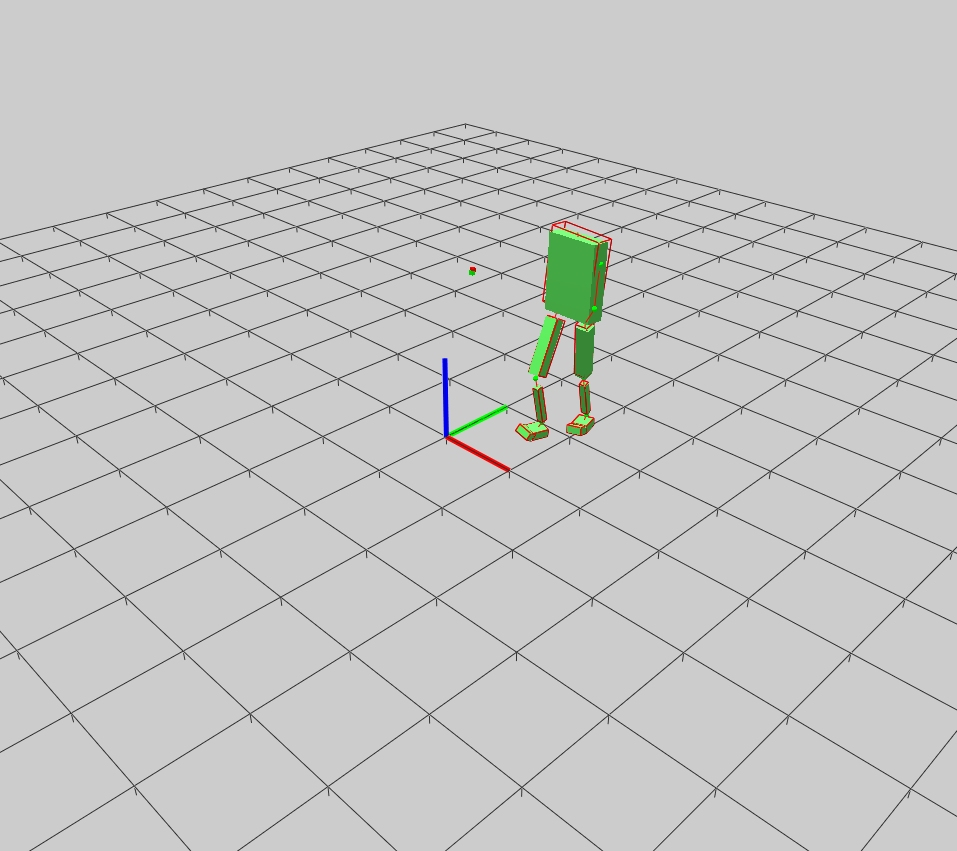
\includegraphics[trim = 70mm 80mm 70mm 50mm, clip, width=1.5in]{pymss/00451}}\\
  \subfloat{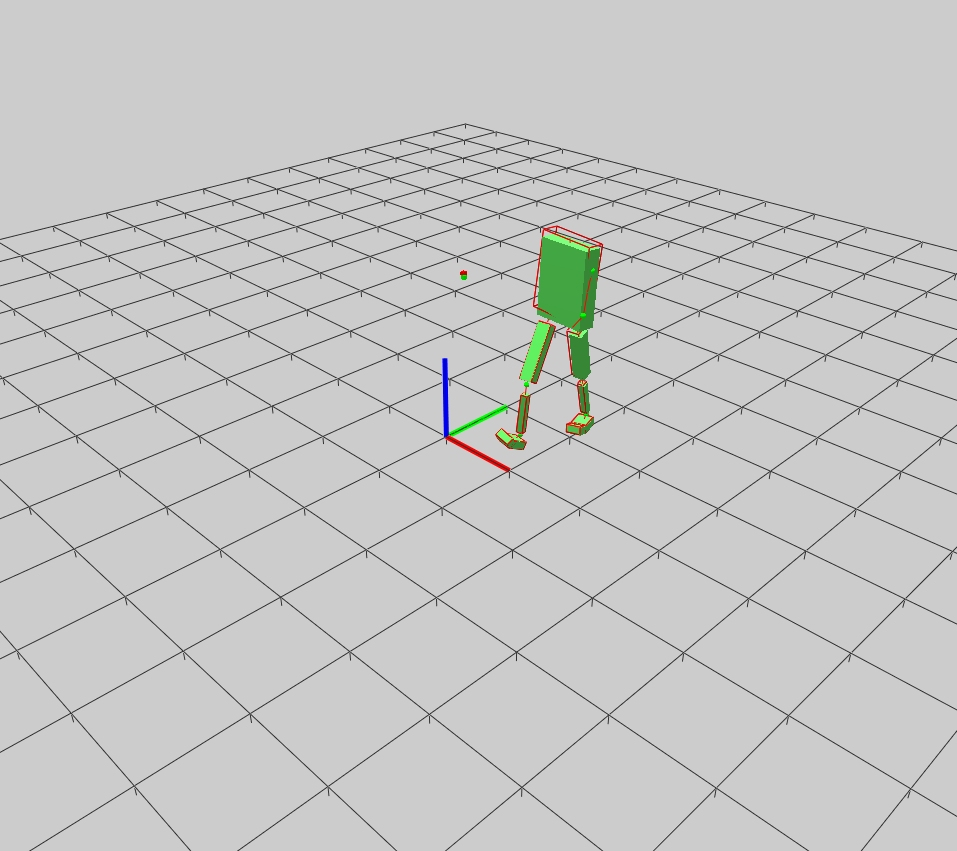
\includegraphics[trim = 70mm 80mm 70mm 50mm, clip, width=1.5in]{pymss/00481}}
  \subfloat{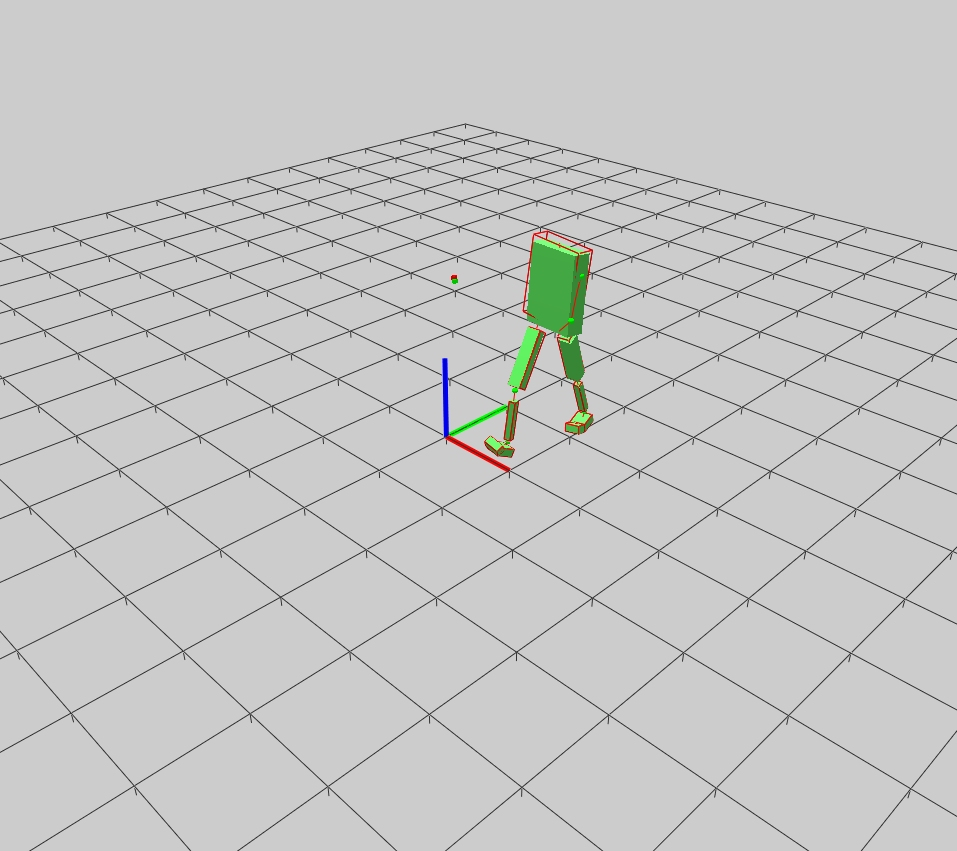
\includegraphics[trim = 70mm 80mm 70mm 50mm, clip, width=1.5in]{pymss/00511}}
  \subfloat{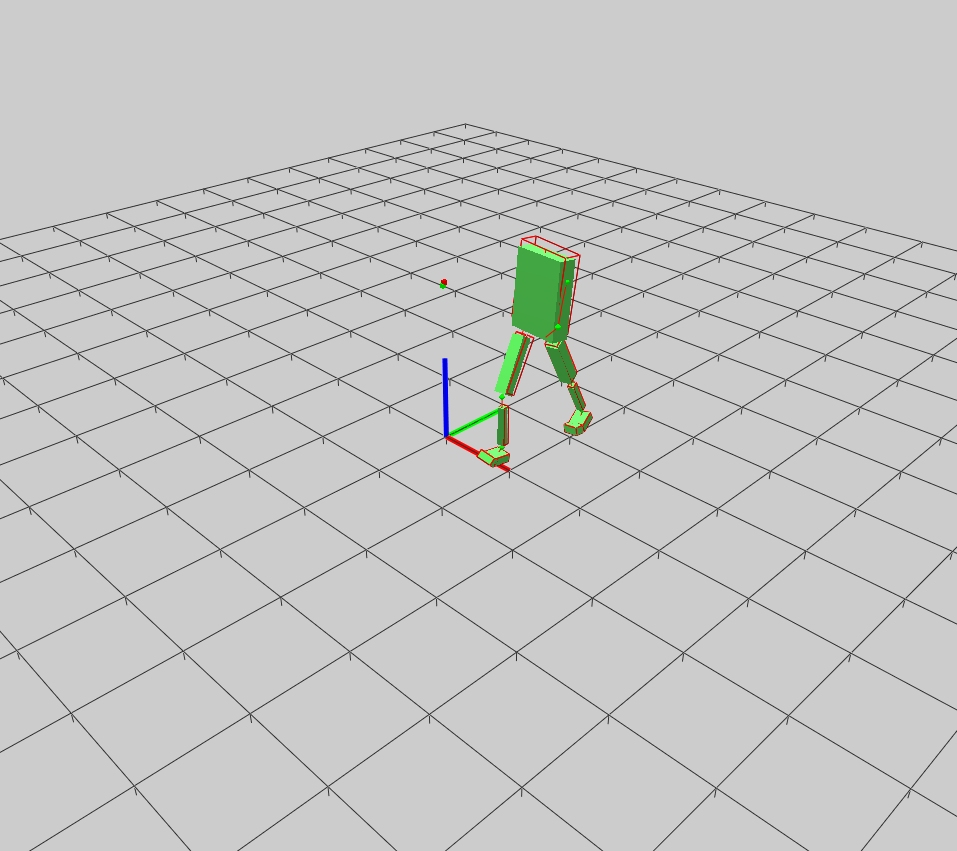
\includegraphics[trim = 70mm 80mm 70mm 50mm, clip, width=1.5in]{pymss/00541}}
  \subfloat{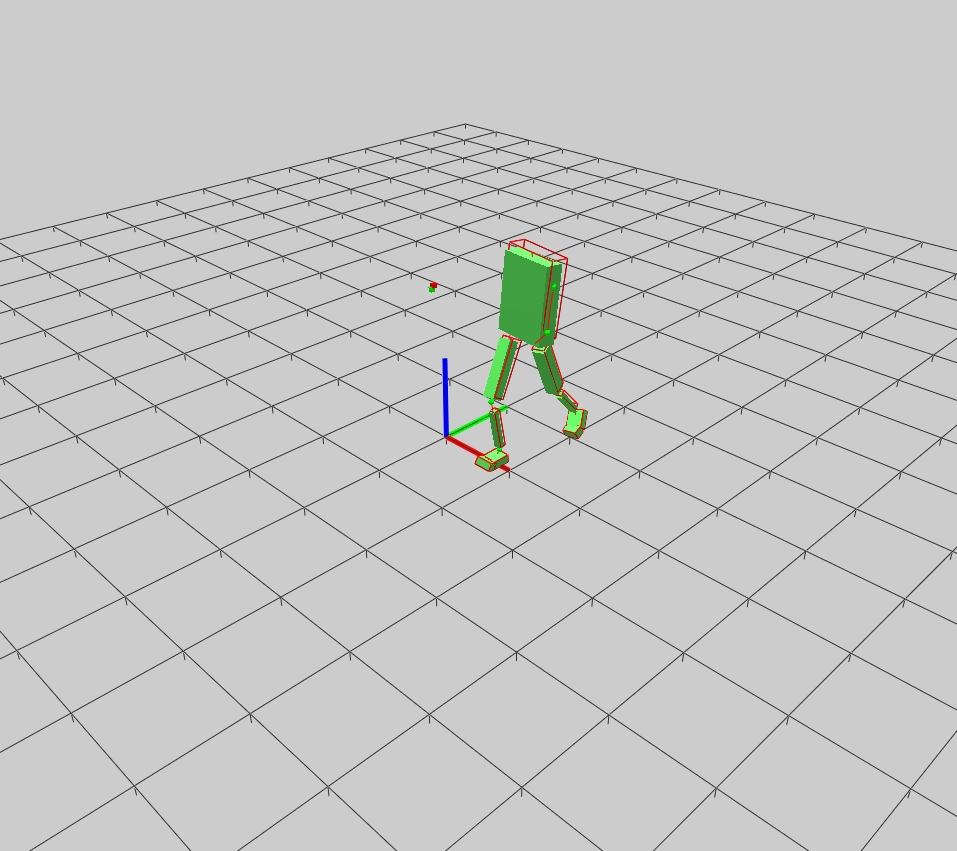
\includegraphics[trim = 70mm 80mm 70mm 50mm, clip, width=1.5in]{pymss/00571}}\\
  \caption{Locomotion snapshots (1 of 2)}
  \label{fig:snapshot1}
\end{figure}

\begin{figure}
  \centering
  \subfloat{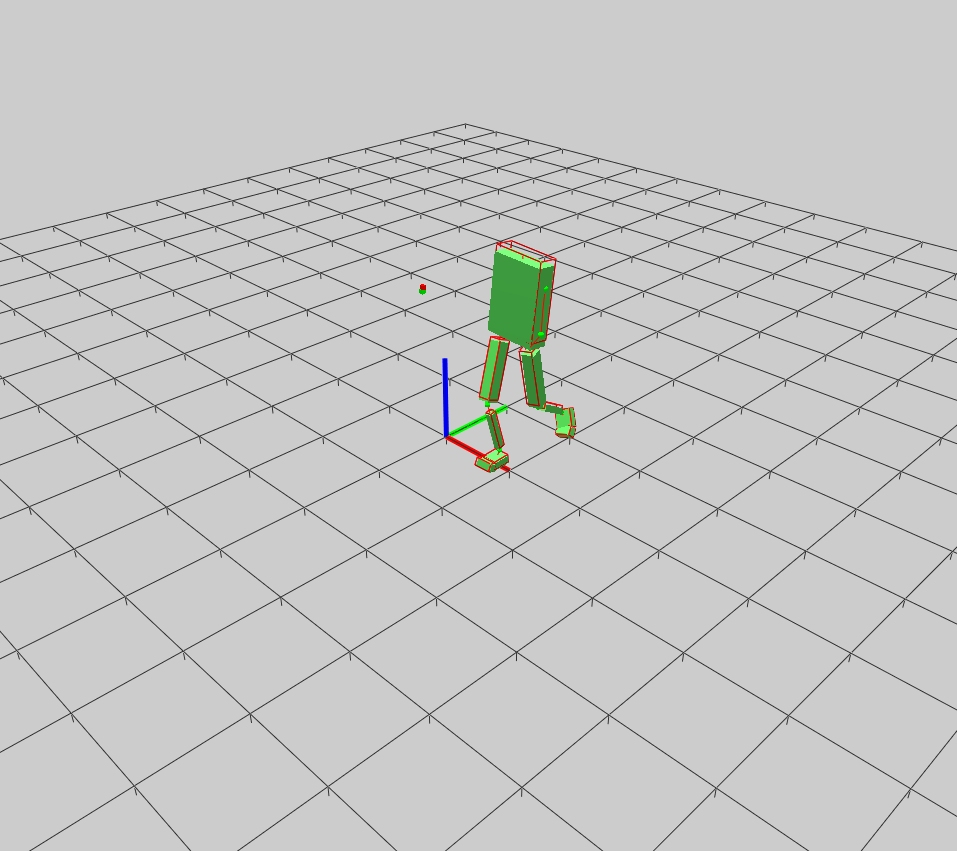
\includegraphics[trim = 70mm 80mm 70mm 50mm, clip, width=1.5in]{pymss/00601}}
  \subfloat{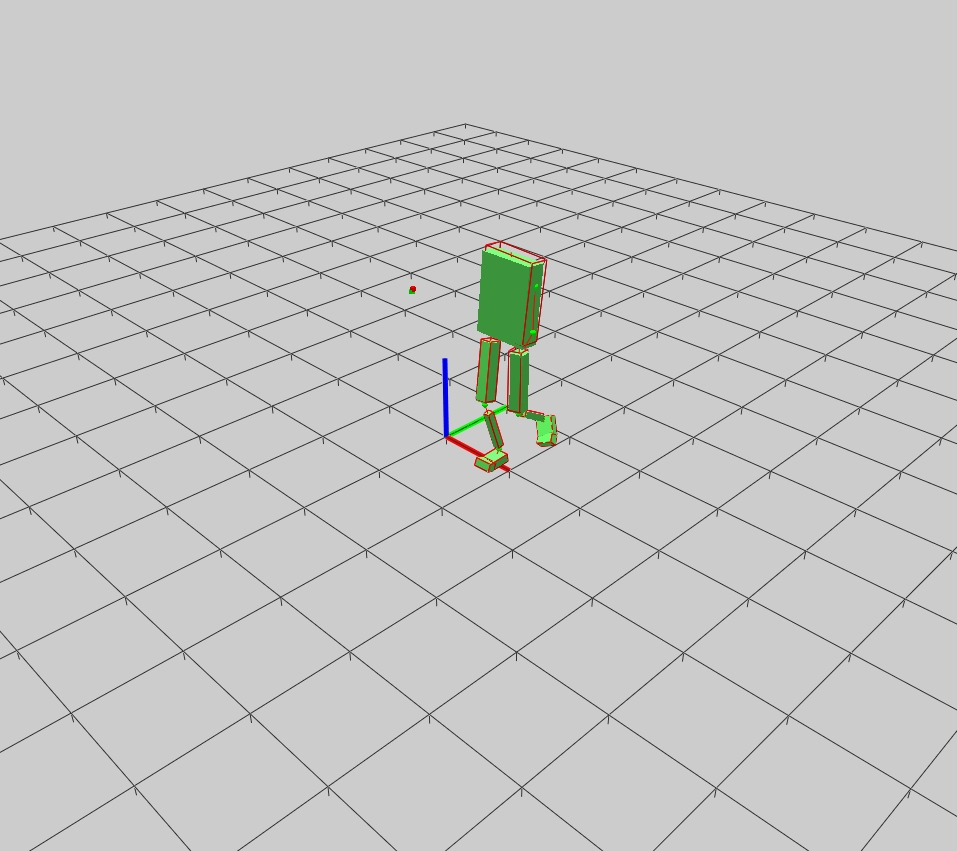
\includegraphics[trim = 70mm 80mm 70mm 50mm, clip, width=1.5in]{pymss/00631}}
  \subfloat{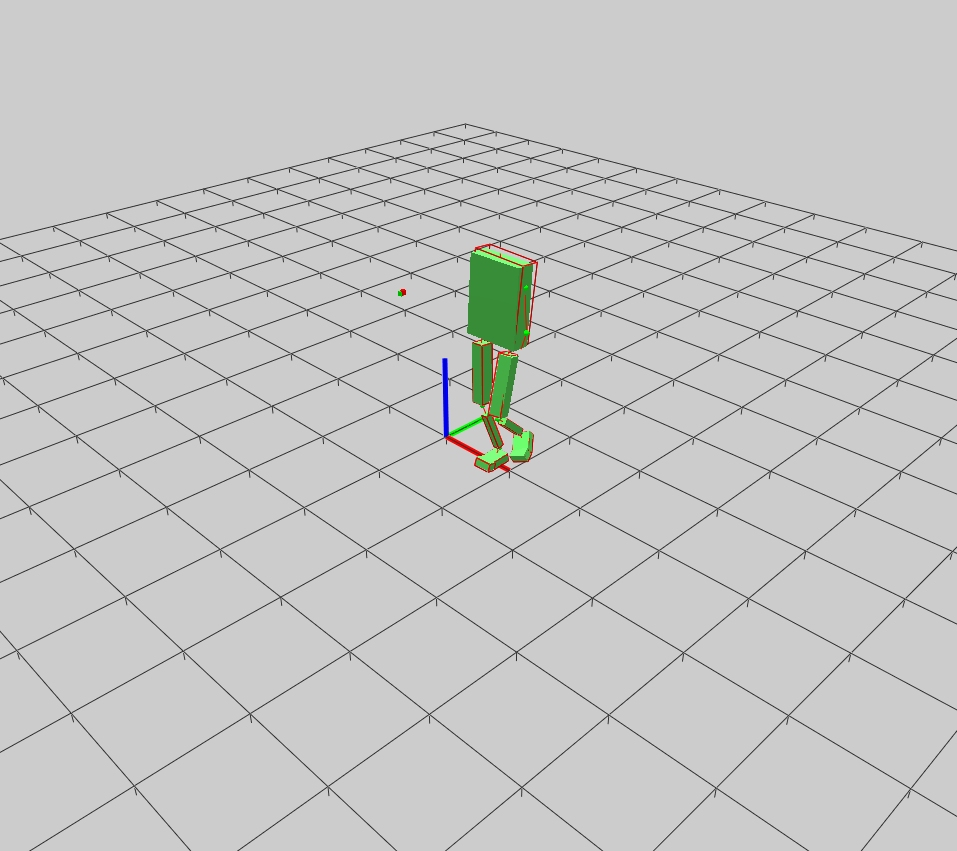
\includegraphics[trim = 70mm 80mm 70mm 50mm, clip, width=1.5in]{pymss/00661}}
  \subfloat{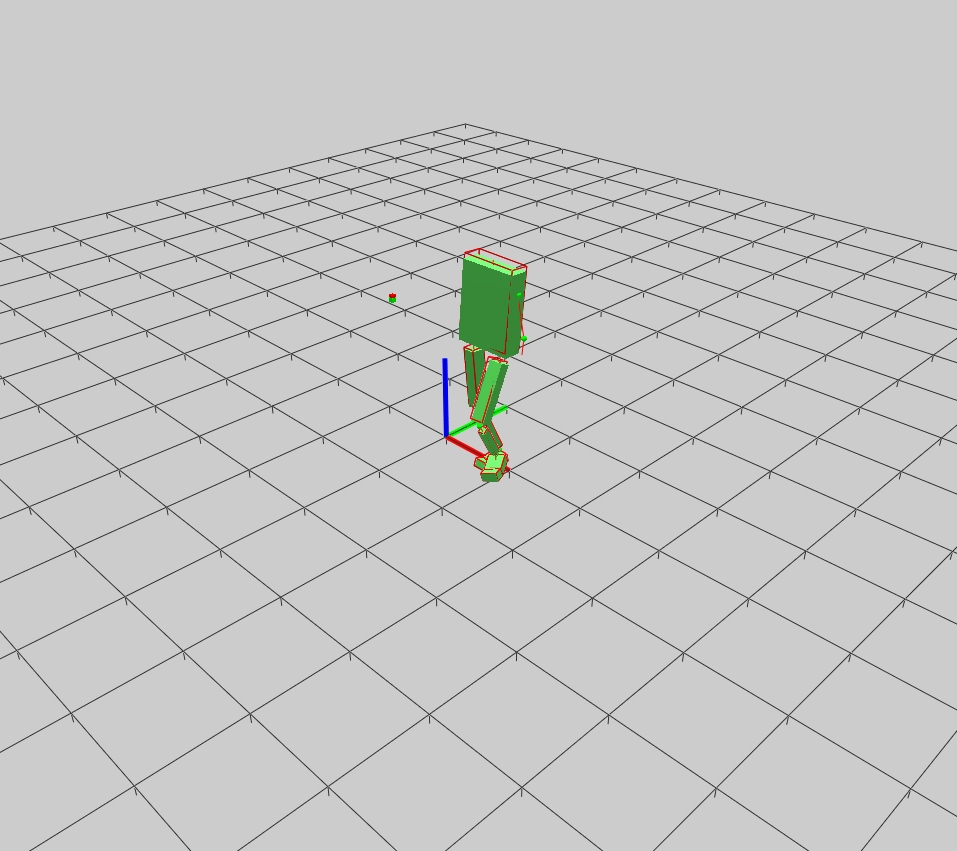
\includegraphics[trim = 70mm 80mm 70mm 50mm, clip, width=1.5in]{pymss/00691}}\\
  \subfloat{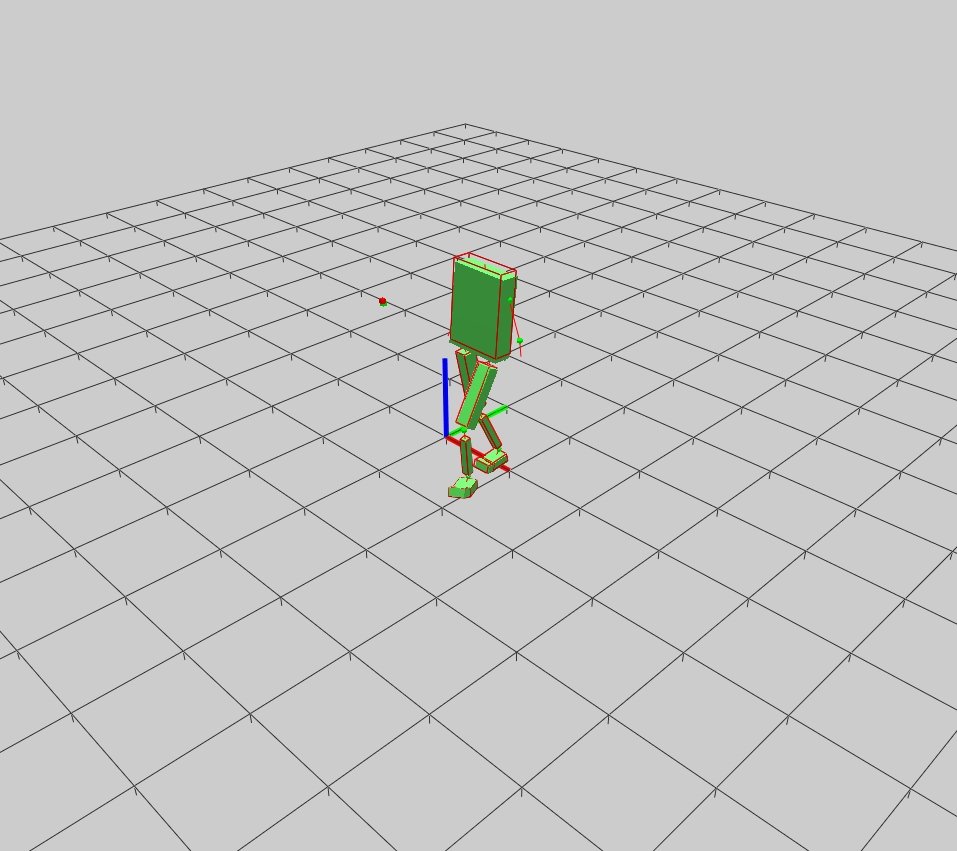
\includegraphics[trim = 70mm 80mm 70mm 50mm, clip, width=1.5in]{pymss/00721}}
  \subfloat{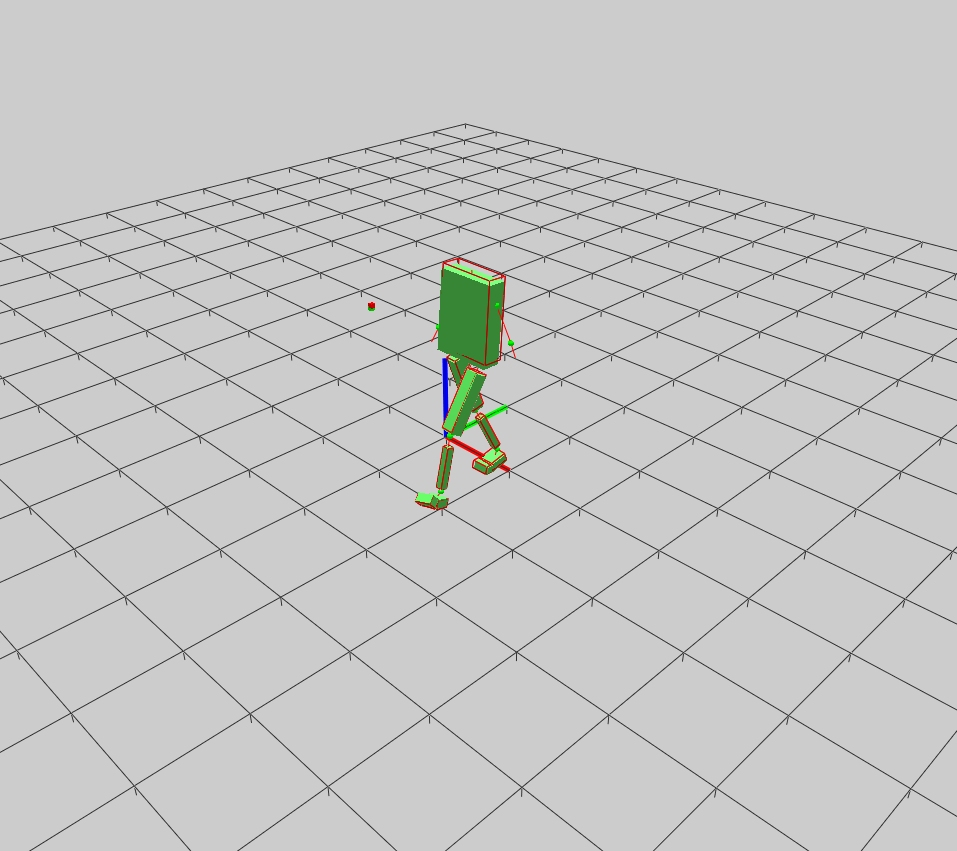
\includegraphics[trim = 70mm 80mm 70mm 50mm, clip, width=1.5in]{pymss/00751}}
  \subfloat{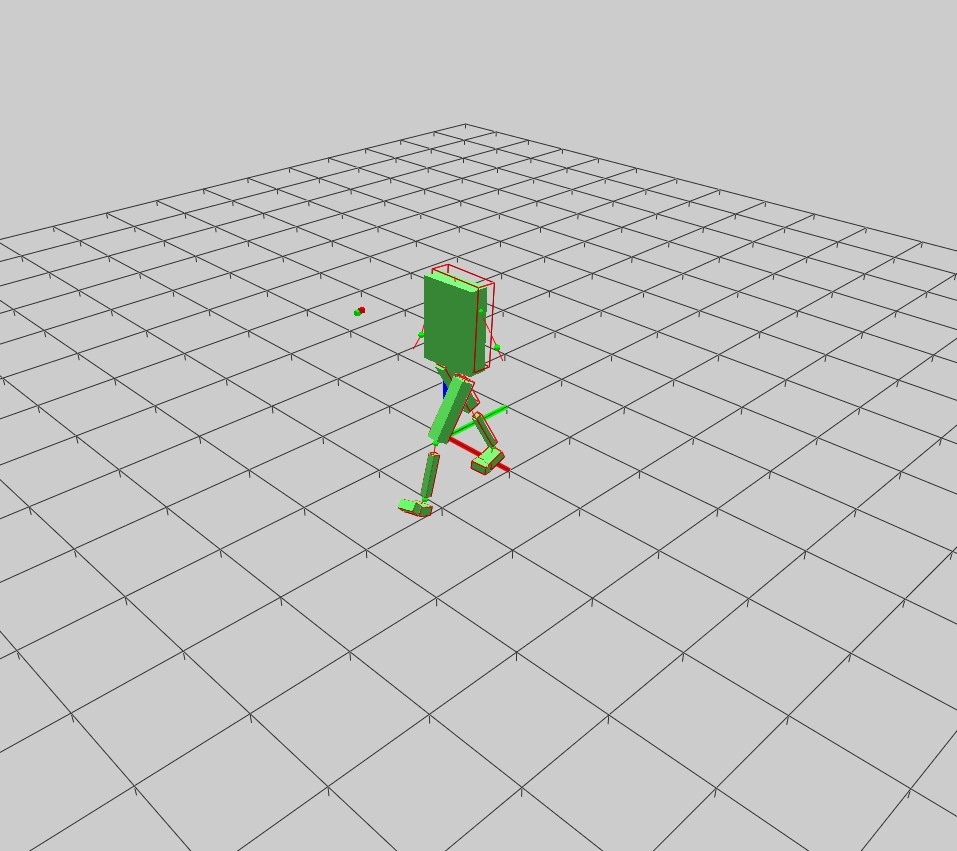
\includegraphics[trim = 70mm 80mm 70mm 50mm, clip, width=1.5in]{pymss/00781}}
  \subfloat{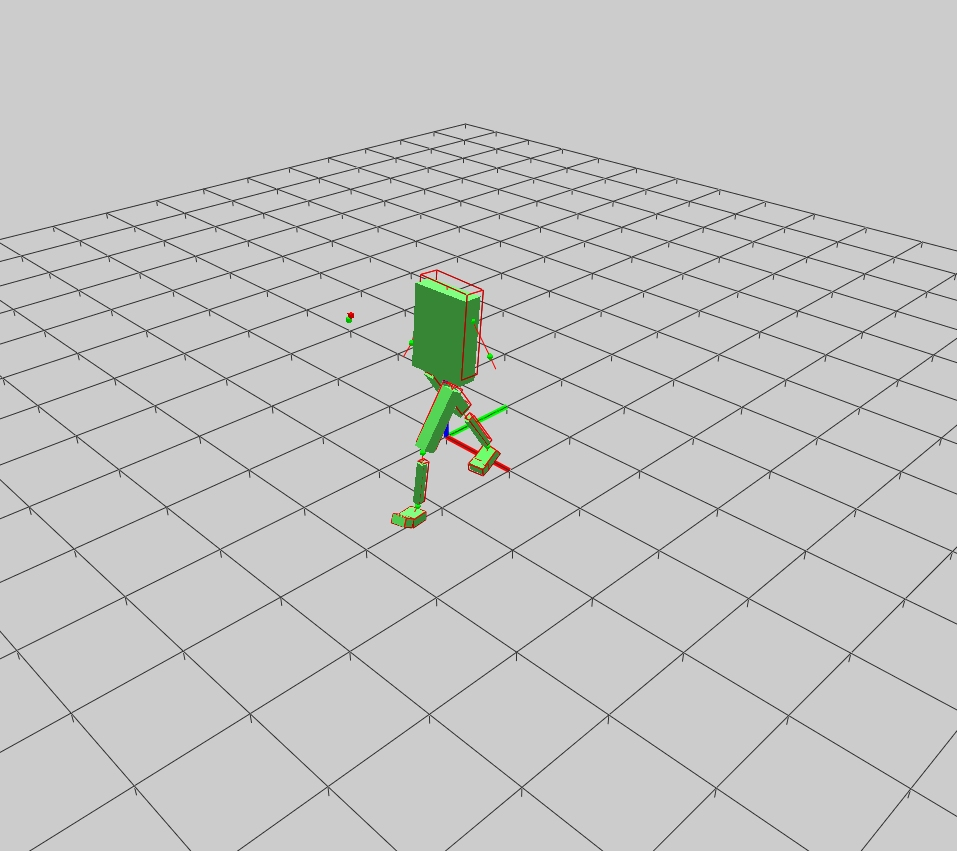
\includegraphics[trim = 70mm 80mm 70mm 50mm, clip, width=1.5in]{pymss/00811}}\\
  \subfloat{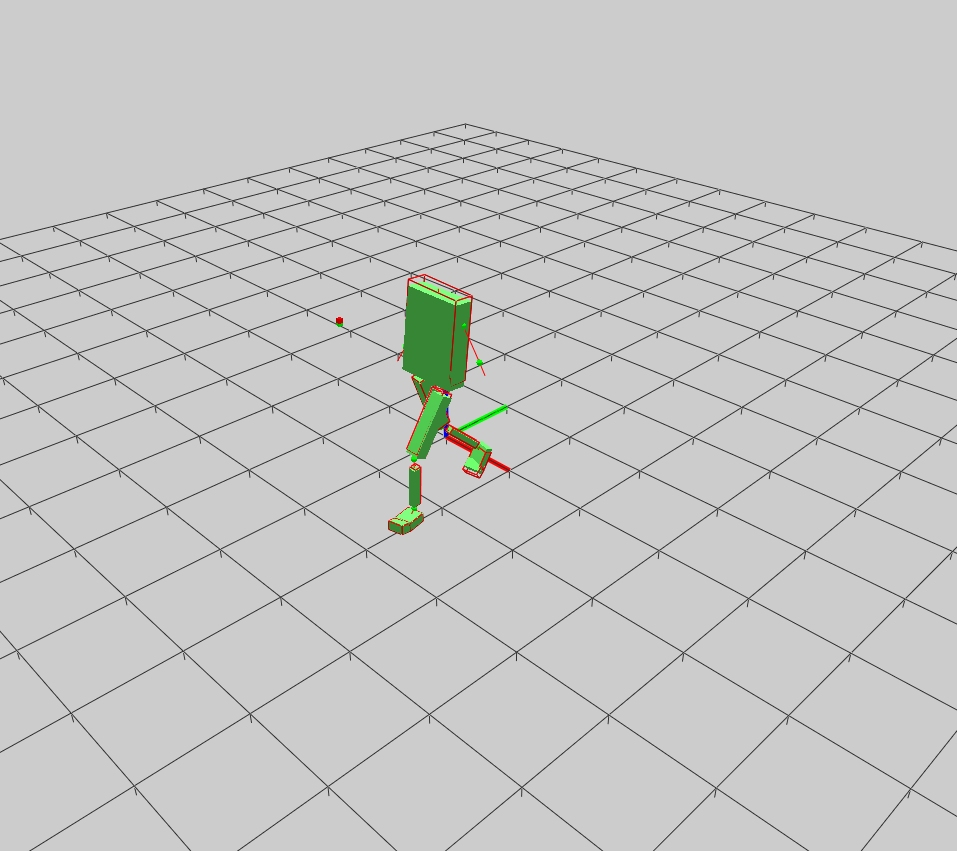
\includegraphics[trim = 70mm 80mm 70mm 50mm, clip, width=1.5in]{pymss/00841}}
  \subfloat{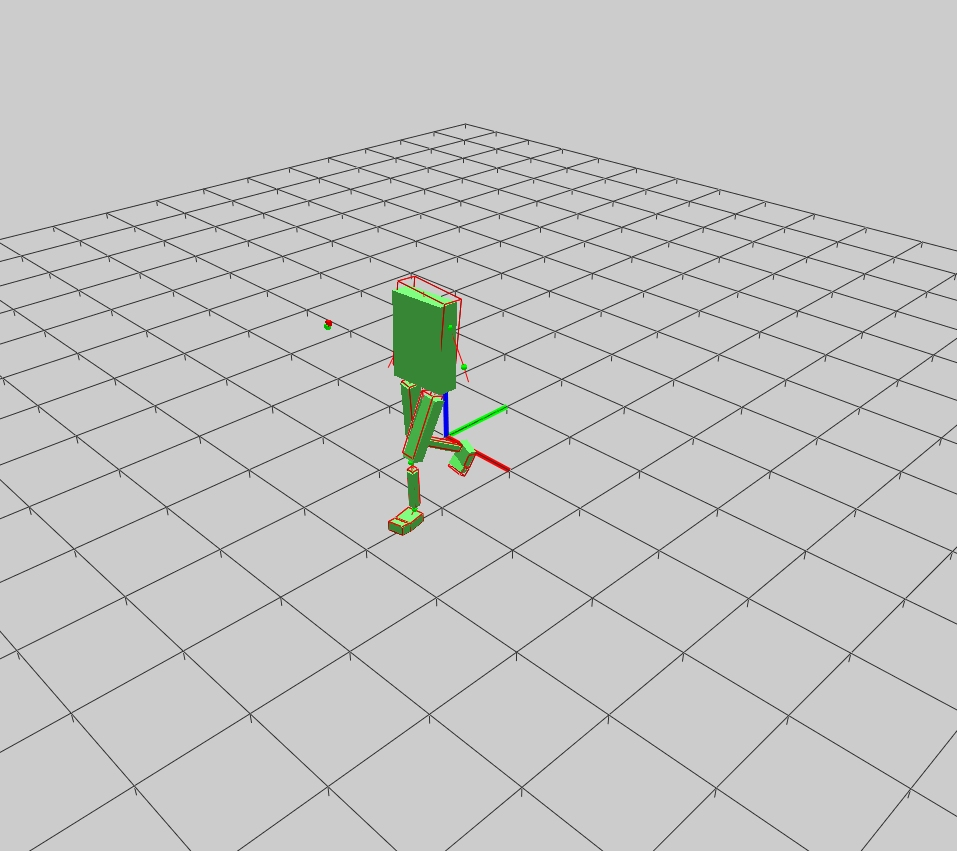
\includegraphics[trim = 70mm 80mm 70mm 50mm, clip, width=1.5in]{pymss/00871}}
  \subfloat{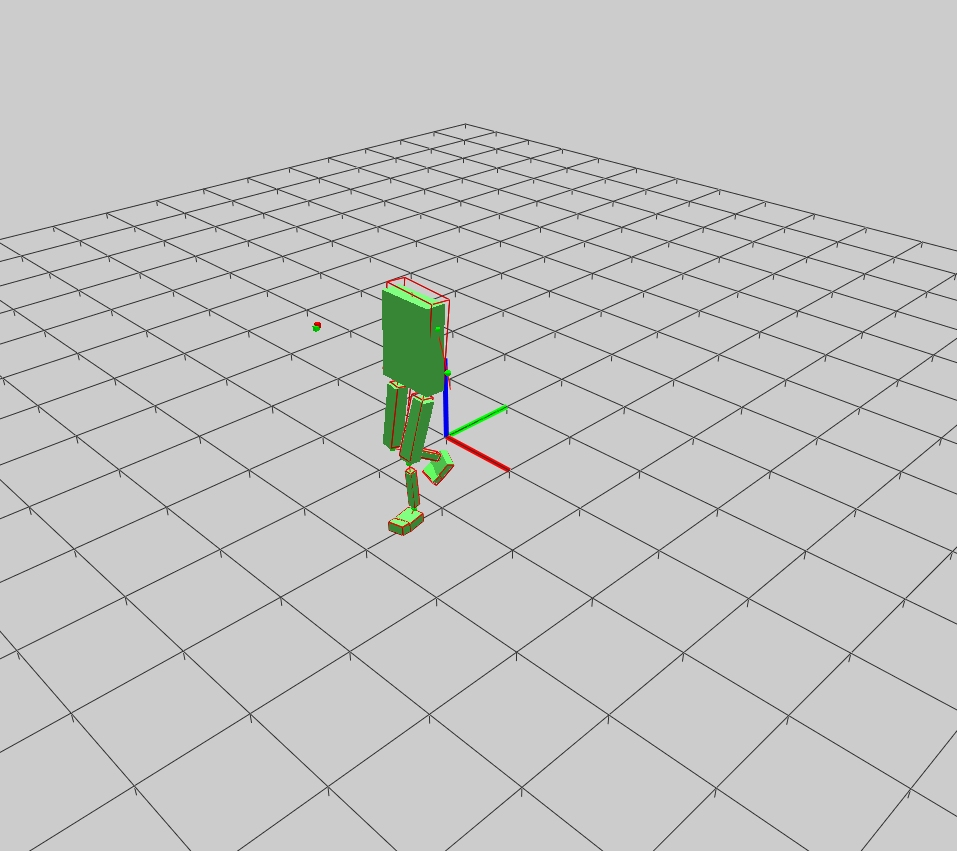
\includegraphics[trim = 70mm 80mm 70mm 50mm, clip, width=1.5in]{pymss/00901}}
  \subfloat{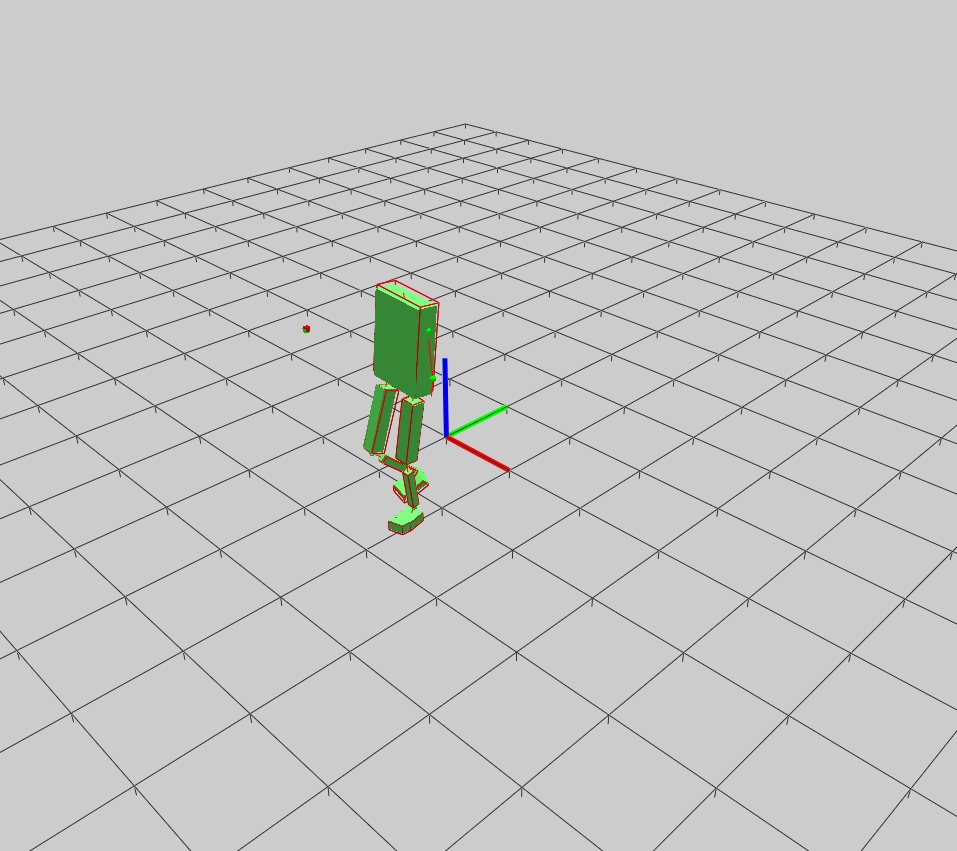
\includegraphics[trim = 70mm 80mm 70mm 50mm, clip, width=1.5in]{pymss/00931}}\\
  \subfloat{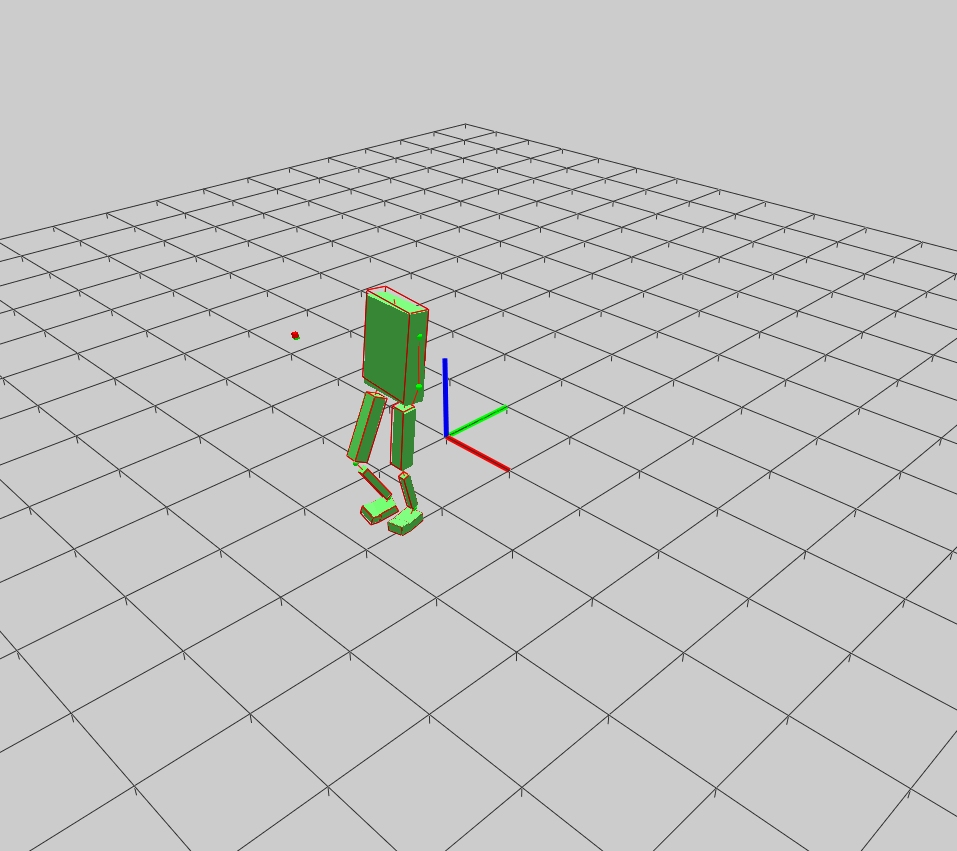
\includegraphics[trim = 70mm 80mm 70mm 50mm, clip, width=1.5in]{pymss/00961}}
  \subfloat{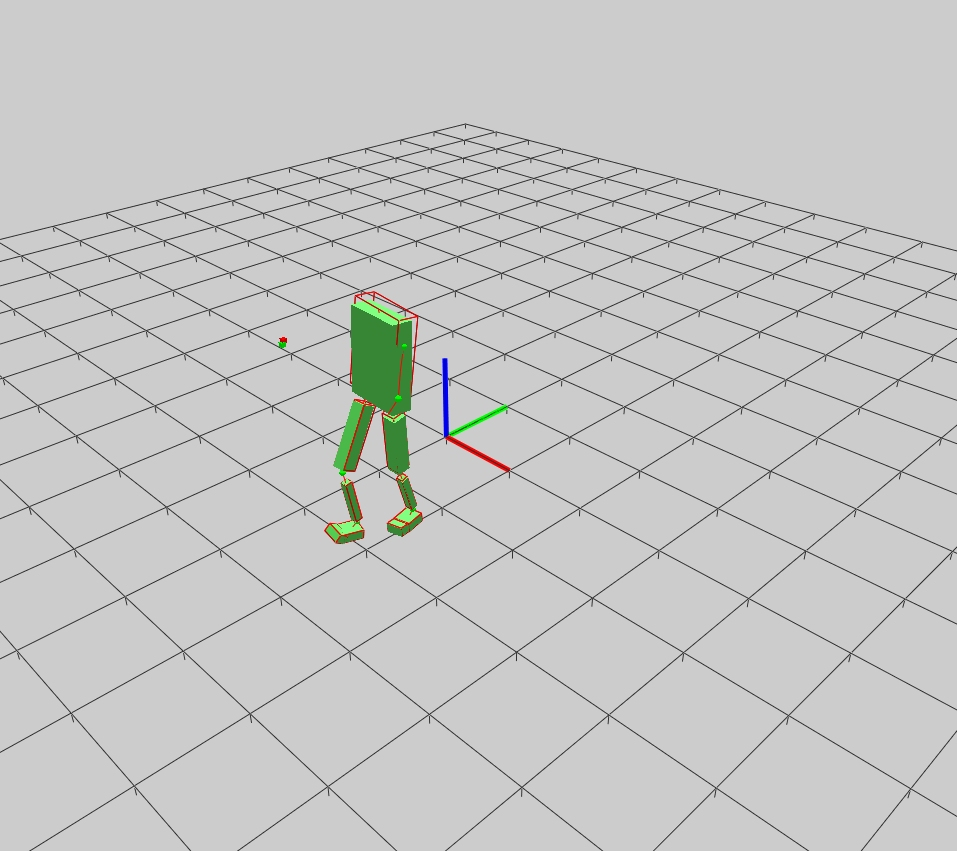
\includegraphics[trim = 70mm 80mm 70mm 50mm, clip, width=1.5in]{pymss/00991}}
  \subfloat{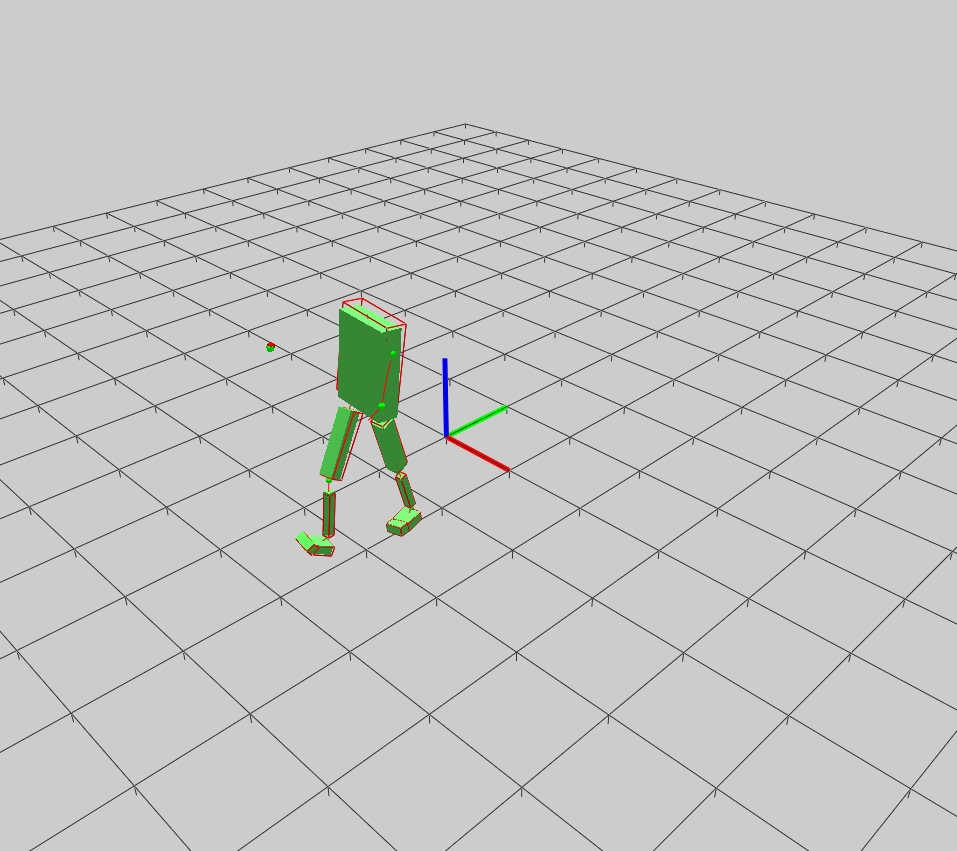
\includegraphics[trim = 70mm 80mm 70mm 50mm, clip, width=1.5in]{pymss/01021}}
  \subfloat{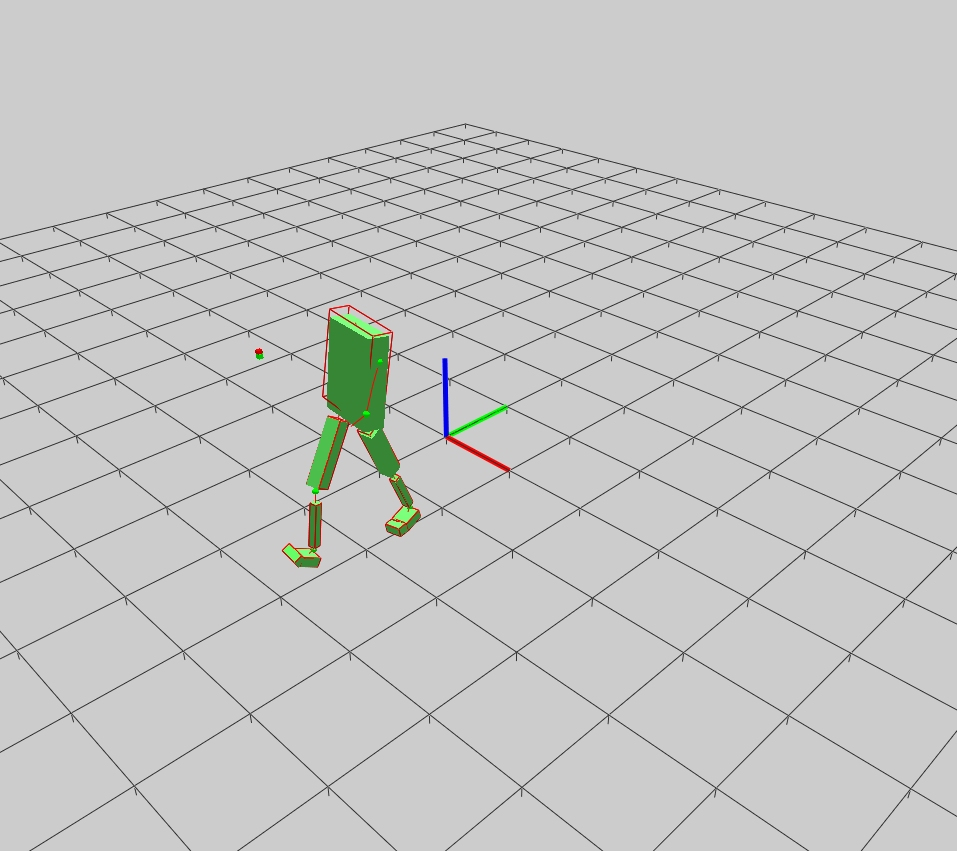
\includegraphics[trim = 70mm 80mm 70mm 50mm, clip, width=1.5in]{pymss/01051}}\\
  \subfloat{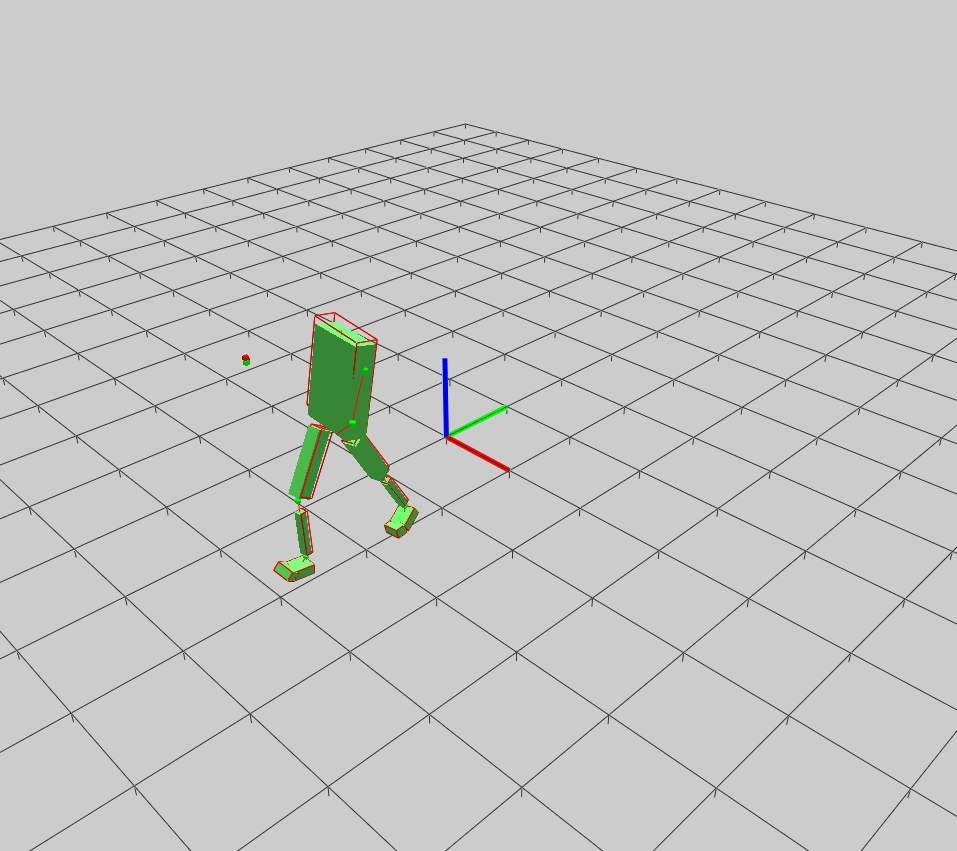
\includegraphics[trim = 70mm 80mm 70mm 50mm, clip, width=1.5in]{pymss/01081}}
  \subfloat{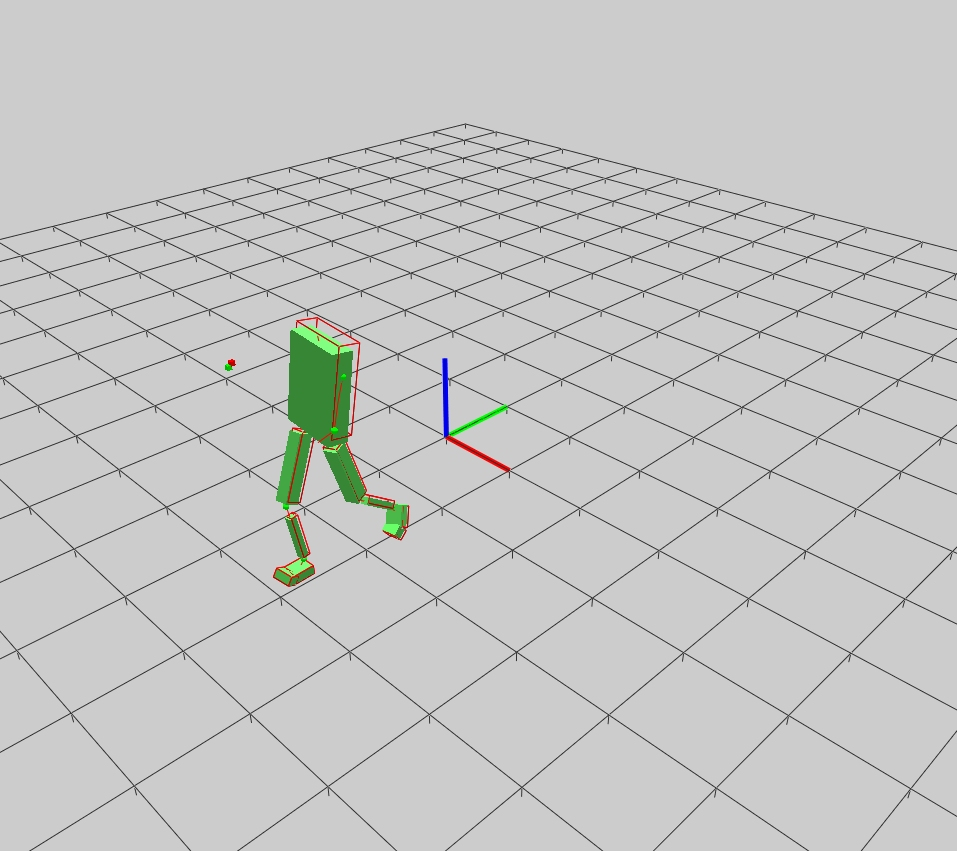
\includegraphics[trim = 70mm 80mm 70mm 50mm, clip, width=1.5in]{pymss/01111}}
  \subfloat{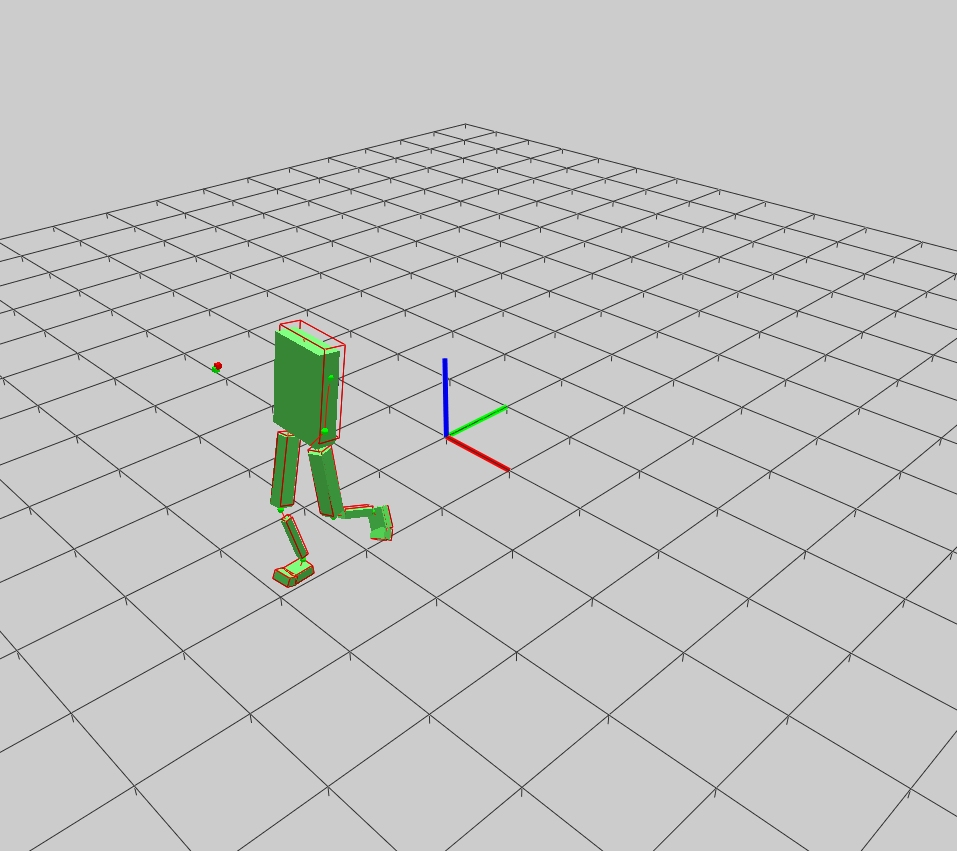
\includegraphics[trim = 70mm 80mm 70mm 50mm, clip, width=1.5in]{pymss/01141}}
  \subfloat{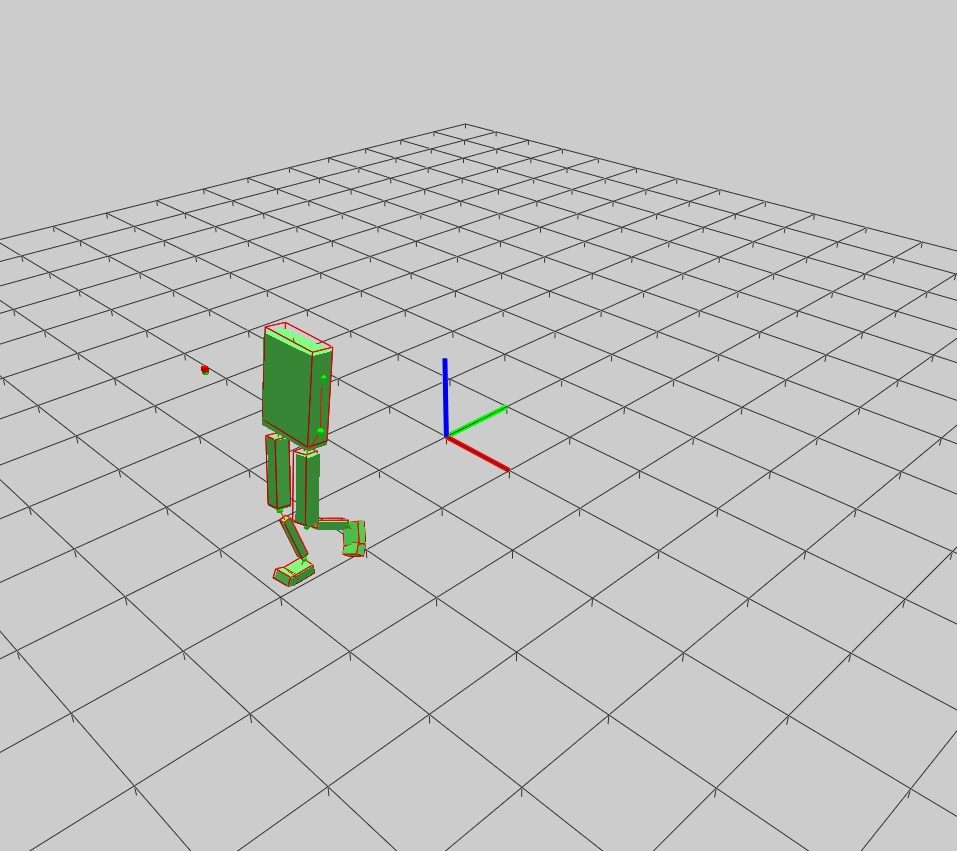
\includegraphics[trim = 70mm 80mm 70mm 50mm, clip, width=1.5in]{pymss/01171}}\\
  \caption{Locomotion snapshots (1 of 2)}
  \label{fig:snapshot2}
\end{figure}

%\begin{figure}[h!]
%  \centering
%  \includegraphics[width=5.in]{reftrack}
%  \caption[Reference tracking performance]
%  {Reference tracking performance: $x$-axis denotes the simulation frame index
%   and $y$-axis denotes $||\chi-\bar{\chi}||$.}
%  \label{fig:devi}
%\end{figure}


%begin{figure}[h!]
% \centering
% \includegraphics[width=2.0in]{penalty}
% \caption{Normal force calculated from the penalty method}
%end{figure}

\chapter{Conclusion}
In this thesis, we proposed a biomechanical biped model
which can be used for synthesizing character animation.
Muscle fibers are used to actuate rigid segments
with tension forces instead of torques exerted from joint motors.
The muscle fibers are attached based on the human
musculoskeletal structure.
Strictly speaking, our biped model is not an articulated system
since there is no rigid joints (articulations). Instead,
we use soft joints to allow joint dislocation.
During optimization, the biped may deliberately
dislocate its body segment within the threshold to achieve
the optimal objective value.
With our proposed biped model, we designed a locomotion tracker
based on optimization.
We computed necessary actuation forces to drive our biomechanical
biped to follow given reference trajectories.

%There has been some work related
%to a realistic human musculoskeletal system for visualization
%in computer graphics, but none of them addresses
%an issue related to biped locomotion and physics simulation.

Although we proposed the biped model based on
human musculoskeletal structure,
we could not evaluated the effects of biomechanical
components.
For instance, we may analyze how energy is efficiently
stored and released in the muscle fiber model.
In a contraction phase, the energy is stored in springs
of the muscle fiber model. On the other hand, the energy released
in an extension phase.
Thus, if actuation forces are exerted on a muscle fiber to contract,
no actuation forces are required to extend the fiber afterwards.
In locomotive motions, this kind of passive dynamics effects has been
vastly observed; however, our optimization formulation was not able to
reflect the biomechanical effects.

%Parameters regarding to soft joints and muscle fibers have
%not been used in previous biped models at all.
%By tweaking model parameters, we synthesized various human
%motions based on motion capture data.

As future work, we propose a locomotion controller in which gait phases
are exploited. Instead of using an optimization, we can design
a proportional-derivative (PD) controller for each phase separately.
Besides, a balancing technique can be adopted to our model such as the strategy
presented in SIMBICON~\cite{journals/tog/YinLP07}. By employing the balancing
scheme, the robustness to external forces during locomotion is expected to be improved.


%Coactivation of muscles.


%%
%% 한글요약문 시작
%%
%% Note. 영문논문일 경우에만 필요하니 한글논문의 경우에는 작성하지 마십시오.
%%
\begin{summary}

캐릭터 애니메이션에 물리 기반 모델은 널리 쓰여 왔다.
캐릭터 애니메이션에 쓰이는 이족 보행 모델은 로봇 공학으로부터 나왔기 때문에
자연스럽게 로봇의 형태와 흡사한 것이 쓰인다.
로봇과 유사한 보편적인 이족 보행 모델에서 각 관절에는 작동시킬 수 있는 발동기가
부착되어, 그 발동기는 로봇이 원하는 자세를 취하도록 제어되어 몸체가 움직이게 된다.

본 논문에서 제안하는 생체 역학적인 이족 보행 모델은
사람의 움직임이 실제 사람에게는 존재하지 않는
발동기가 아닌 골격 구조에 부착된 근섬유의 장력으로 인해
제어된다는 착안에 기반한다.
이 모델에서는 사람의 신체 각 부분을 강체로 모형화시키고,
강체에 근섬유 모형을 부착시킴으로써 사람의 근골격 구조를
설계했다. 또한, 각 관절의 연골을 모형화시켜서 어느 정도의
탈골을 허용하도록 관절 구조를 모형화시켰다.

이러한 생체 역학적 이족 보행 모델에 기반하여
주어진 동작 포착 자료를 추적하는 추적기를 설계한다.
이 추적기는 주어진 동작을 따라하기 위해 필요한 최적의 근섬유 힘을 계산한다.
몇 가지 일반적인 보행 동작에 대해 제안된 모델과 최적화 기반 추적기가
작동 하는 것을 시뮬레이션을 통해 보인다.

\noindent
\\핵심어: 캐릭터 애니메이션, 동역학, 이족 보행 모델, 생체 역학
\end{summary}

%%
%% 참고문헌 시작
%%
\bibliographystyle{IEEETrans}
\bibliography{muscle.bib}

%%
%% 감사의 글 시작
%%

\acknowledgement

석사 생활을 마치며 가장 떠오르고 또한 감사를 드리고 싶은 분은 저의 지도교수님이신
신성용 교수님입니다. 저에게 연구란 어떤 것인지, 연구자의 자세란 어떤 것인지
머리가 아닌 마음으로 느낄 수 있게 해 주셨습니다. 저에게 항상 최고의 것만을
주시려고 애써주시고, 또한 저의 진로에 대해서 항상 걱정해 주시고,
또 기대해 주심에 글로는 다 표현 못할 감사를 드립니다.

언제까지나 함께일 것만 같았던 영상이형, 내진이형, 상욱이형, 다성이형,
동훈이형, 일우형, 상호과 곧 헤어질 것을 생각하니 벌써부터 눈물이 앞을 가립니다.
연구하다가 막막한 점이 있을 때 자기 일처럼 도와주시던 다성이형에게 특별히 고마움을 전합니다.
지금은 연구실에 없는 나협이형, 정환이형,
민혁이 모두 길지 않은 시간이었지만 정말 소중한 인연이었습니다.
비록 같은 연구실은 아니었지만 석사 과정 동기로 만나게 되어
전산학을 향한 순수한 열정을 함께 공유한 현종이형에게도 고맙다는 말을
전합니다.

%
%%
%% 이력서 시작
%%
% @command curriculumvitae 이력서
% @options [default: 클래스 옵션 korean|english ]
% - korean : 한글이력서 | english : 영문이력서
\curriculumvitae[korean]

    % @environment personaldata 개인정보
    % @command     name         이름
    %              dateofbirth  생년월일
    %              birthplace   출생지
    %              domicile     본적지
    %              address      주소지
    %              email        E-mail 주소
    % - 위 6개의 기본 필드 중에 이력서에 적고 싶은 정보를 입력
    \begin{personaldata}
        \name       {김 거 엽}
        \dateofbirth{1985}{5}{6}
        %\birthplace {서울 영등포구 영등포동 ...}
        %\domicile   {대전 유성구 신성동 ...}
        \address    {서울특별시 관악구 봉천동 복권아파트 3동 305호}
        \email      {gb@jupiter.kaist.ac.kr}
    \end{personaldata}

    % @environment education 학력
    % @options [default: (none)] - 수학기간을 입력
    \begin{education}
        \item[2001. 3.\ --\ 2004. 2.] 여의도고등학교
        \item[2004. 3.\ --\ 2008. 8.] 연세대학교 전기전자공학부 (B.S.)
        \item[2008. 9.\ --\ 2011. 2.] KAIST 전산학과 (M.S.)
    \end{education}

    % @environment career 경력
    % @options [default: (none)] - 해당기간을 입력
    %\begin{career}
    %    \item[2010. 2.\ --\ 2010. 12.] 프로그래밍 기초 (CS101) 조교
    %\end{career}

    % @environment activity 학회활동
    % @options [default: (none)] - 활동내용을 입력
    %\begin{activity}
        %\item J. Choi, \textbf{Yong-Hyun Kim}, K.J. Chang, and D. Tomanek,
        %     \textit{Occurrence of itinerant ferromagnetism in C/BN superlattice
        %     nanotubes}, 5th Asian Workshop on First-Principles Electronic
        %     Structure Calculations, Seoul (Korea), October., 2002.
    %\end{activity}

    % @environment publication 연구업적
    % @options [default: (none)] - 출판내용을 입력
    %\begin{publication}
        %\item \textbf{Yong-Hyun Kim}, J. Choi, K.J. Chang, and D. Tomanek,
        %     \textit{Magnetic instability in partly opened C$_{60}$ isomers},
        %     in preparation.
    %\end{publication}



%% 본문 끝

%\end{CJK*}
\end{document}
